% ============================================================
%  Paper 5 — The Grand Unification:
%  Γ as Universal Interface Law and C2 as Universal Remodeling
% ============================================================
\documentclass[aps,pre,twocolumn,superscriptaddress,floatfix]{revtex4-2}

\usepackage{amsmath,amssymb,amsthm,bm,graphicx,booktabs,multirow,siunitx,hyperref}
\hypersetup{colorlinks=true,linkcolor=blue,citecolor=blue,urlcolor=blue}

\newtheorem{theorem}{Theorem}
\newtheorem{proposition}{Proposition}
\newtheorem{corollary}{Corollary}
\newtheorem{remark}{Remark}

\newcommand{\Aimp}{A_{\text{imp}}}
\newcommand{\Acut}{A_{\text{cut}}}

\begin{document}

\title{Paper~5: The Grand Unification---$\Gamma$ as the
Universal Interface Law from Microtubules to Power Grids,
and C2 as Universal Remodeling in Twenty-Nine Tissues}

\author{Hsi-Yu Huang}
\email{llc.y.huangll@gmail.com}
\affiliation{Independent Researcher, Taipei, Taiwan}

\date{\today}


% ============================================================
%  ABSTRACT
% ============================================================
\begin{abstract}
Papers~1--4 developed $\Gamma$-Net physics for neural,
vascular, temporal, and consciousness phenomena.
This paper establishes two grand-unification results.

\textbf{Part~A} resolves the circularity objection
by deriving the reflection coefficient
$\Gamma = (Z_2 - Z_1)/(Z_2 + Z_1)$ and the conservation
identity $\Gamma^2 + T = 1$ from the First Law of
Thermodynamics alone.
NHANES validation (3~cycles, $n = 7{,}393$; 10~cycles,
$n = 49{,}774$; zero fitted parameters; SHA-256
hash-locked) confirms organ-level $\Gamma$-diagnostics
in 7/7 systems (endocrine AUC~$= 0.78$) and all-cause
mortality AUC~$= 0.705$.
An Interface Scale Table spanning 25~nm (microtubules)
to $10^6$~m (ionospheric waveguides) and an interface
isomorphism theorem demonstrate that $\Gamma$ governs
every energy-carrying interface regardless of substrate.

\textbf{Part~B} proves that constraint~C2 (impedance
remodeling, $\Delta Z = -\eta\,\Gamma\,x_{\text{in}}
\cdot x_{\text{out}}$) is the unique gradient-descent
rule for minimising reflected energy at any repeatedly
stimulated interface, then shows that twenty-nine known
remodeling laws---Hebb (neural), Wolff (bone), Glagov
(vascular), Davis (muscle), immune memory, keratinisation,
altitude adaptation, intestinal adaptation, receptor
regulation, lymph node hypertrophy, tubuloglomerular
feedback, liver regeneration, tendon remodeling, leptin
signalling, erythropoiesis, follicular selection,
Laplace--Starling (cardiac), baroreceptor resetting
(regulatory brain),
IOP homeostasis (ocular), tonotopic plasticity (auditory),
VOR adaptation (vestibular), receptor turnover (olfactory),
tertiary dentinogenesis (dental), enteric plasticity,
sympathovagal remodeling (autonomic),
$\beta$-cell compensation (pancreatic),
choroid regulation (CSF),
cortical map plasticity (brain functional),
plus the C2 null case of cartilage
($\eta \approx 0 \Rightarrow$ osteoarthritis)---are
each algebraically equivalent to C2 under the appropriate
substitution of effort, flow, and impedance variables.

NHANES 10-cycle network-propagation validation ($n=49{,}774$,
zero fitted parameters) confirms that a vascular measurement
(blood pressure) improves non-vascular organ predictions
(cardiac $\Delta\text{AUC} = +0.166$, neurological $+0.061$,
renal $+0.024$) through inter-network $\Gamma$-coupling,
while the control organ (endocrine, $\Delta = 0.000$) is
invariant---the empirical signature of network propagation.
\end{abstract}

\maketitle


% ############################################################
%  PART A — Γ AS UNIVERSAL INTERFACE LAW
% ############################################################
\part*{Part A: $\Gamma$ as Universal Interface Law}


% ============================================================
%  SECTION 1 — INTRODUCTION
% ============================================================
\section{Introduction}
\label{sec:intro}

A persistent objection to the $\Gamma$-Net framework
runs as follows: ``You \emph{assume} that biological
interfaces obey $\Gamma = (Z_2-Z_1)/(Z_2+Z_1)$, then
find that the mathematics is self-consistent.  This
proves nothing beyond the coherence of your own
definitions.''

This paper resolves the circularity by establishing
three independent results that do not presuppose
the $\Gamma$-Net axioms:

\begin{enumerate}
  \item \textbf{Derivation from the First Law.}
    We show that $\Gamma$ and the conservation identity
    $\Gamma^2 + T = 1$ are the \emph{unique} consequence
    of applying energy conservation to any one-dimensional
    interface.  No biological modelling is required.

  \item \textbf{External empirical validation.}
    We apply the framework to NHANES population health data
    (3-cycle $n = 7{,}393$; 10-cycle $n = 49{,}774$)
    with zero fitted parameters and SHA-256 hash-locking.
    The predictions are non-trivially correct across
    7~organ systems and all-cause mortality.

  \item \textbf{Scale universality.}
    We present an Interface Scale Table spanning 25~nm
    to $10^6$~m, showing that $\Gamma$ governs energy
    transfer at every scale from microtubule ion transport
    to planetary waveguide propagation.
\end{enumerate}

Together, these results convert the $\Gamma$-Net framework
from a model of neuroscience with three axioms into a
\emph{deductive chain} from the First Law of Thermodynamics.


% ============================================================
%  SECTION 2 — Γ AS THERMODYNAMIC NECESSITY
% ============================================================
\section{$\Gamma$ as Thermodynamic Necessity}
\label{sec:necessity}

\subsection{Definition of generalised impedance}

Consider any interface at which a flow of energy,
matter, or information passes from medium~1 to medium~2.
Define the generalised impedance of medium~$k$ as
\begin{equation}
  Z_k \;=\; \frac{\text{effort}_k}{\text{flow}_k}\,,
  \label{eq:impedance-def}
\end{equation}
where ``effort'' and ``flow'' are the conjugate pair
whose product equals power ($P = \text{effort} \times
\text{flow}$).

\begin{theorem}[Universality of $\Gamma$]
\label{thm:gamma}
At any one-dimensional interface between media of
impedance $Z_1$ and $Z_2$, subject only to energy
conservation (the First Law), the power reflection
and transmission coefficients are:
\begin{align}
  \Gamma &= \frac{Z_2 - Z_1}{Z_2 + Z_1}\,,
  \label{eq:gamma-def}\\
  T &= 1 - \Gamma^2
    = \frac{4\,Z_1\,Z_2}{(Z_1+Z_2)^2}\,.
  \label{eq:T-def}
\end{align}
\end{theorem}

\begin{proof}
Decompose the incident power $P_{\text{in}}$ at the
interface into reflected ($P_r$) and transmitted ($P_t$)
components.  Energy conservation requires
$P_{\text{in}} = P_r + P_t$.
Continuity of effort and flow at the boundary yields:
$\text{effort}_{\text{inc}} + \text{effort}_{\text{ref}}
= \text{effort}_{\text{trans}}$,
$\text{flow}_{\text{inc}} - \text{flow}_{\text{ref}}
= \text{flow}_{\text{trans}}$.
Solving for the amplitude reflection coefficient
$r = \text{effort}_{\text{ref}} /
\text{effort}_{\text{inc}}$:
\[
  r = \frac{Z_2 - Z_1}{Z_2 + Z_1}\,.
\]
The power reflection coefficient is $\Gamma^2 = r^2$,
and $T = 1 - \Gamma^2$ follows from the First Law
($P_r + P_t = P_{\text{in}}$).
\end{proof}

\subsection{The Minimum Reflection Principle as
thermodynamic viability}

Theorem~\ref{thm:gamma} establishes that at any
interface, a fraction $\Gamma^2$ of incident power is
reflected (wasted).
For an organism with $N$ interface channels, the total
reflected power is:
\begin{equation}
  P_{\text{waste}} = \sum_{i=1}^N \Gamma_i^2\,P_{\text{in},i}\,.
  \label{eq:waste}
\end{equation}
An organism is \emph{thermodynamically viable} if and only if
\begin{equation}
  P_{\text{metabolic}} > P_{\text{waste}}\,,
  \label{eq:viability}
\end{equation}
i.e., its metabolic power production exceeds its
reflection losses.  Organisms that violate
Eq.~\eqref{eq:viability} die by energy deficit---no
natural-selection argument required.

The Minimum Reflection Principle (MRP) is therefore not
an optimality \emph{assumption} but a thermodynamic
\emph{viability condition}: organisms that waste too much
energy at their interfaces fail by physics alone, before
selection has a chance to act.

\subsection{C2 as gradient descent on the reflection action}

Define the reflection action over lifetime~$T$:
\begin{equation}
  \mathcal{A}[\Gamma]
  = \int_0^T \sum_i \Gamma_i^2(t)\,P_{\text{in},i}(t)\,dt\,.
  \label{eq:action}
\end{equation}
First-order gradient descent on $\mathcal{A}$ with
respect to $Z_i$, gated by input and output activity,
yields:
\begin{equation}
  \boxed{
  \Delta Z_i = -\eta\,\Gamma_i\,x_{\text{in},i}
  \cdot x_{\text{out},i}
  }
  \quad\text{(C2: impedance remodeling)}\,,
  \label{eq:C2}
\end{equation}
which is constraint~C2 of the $\Gamma$-Net framework.
This is not a postulate: it is the \emph{unique}
first-order activity-gated update rule that minimises
reflected energy.


% ============================================================
%  SECTION 3 — NHANES VALIDATION
% ============================================================
\section{Empirical Validation: NHANES}
\label{sec:nhanes}

\subsection{Three-cycle blind validation}
\label{sec:nhanes-3cycle}

\subsubsection{Protocol}

We test the framework on real human data:
NHANES 2013--2018 ($n = 7{,}393$).
The protocol is:
\begin{enumerate}
  \item Define organ impedance from textbook physiology:
    $Z_{\text{organ}} = \sum_j w_j\,|x_j - x_{\text{ref},j}|
    / x_{\text{ref},j}$.
  \item Define organ $\Gamma$:
    $\Gamma_{\text{organ}} = (Z_{\text{patient}} -
    Z_{\text{normal}}) / (Z_{\text{patient}} +
    Z_{\text{normal}})$.
  \item Hash-lock the entire pipeline (SHA-256) before
    accessing outcome data.
  \item Predict organ disease status
    ($\Gamma_{\text{organ}}^2 > \theta$).
  \item Compare with self-reported diagnoses.
  \item Zero fitted parameters throughout.
\end{enumerate}

\subsubsection{Results}

\begin{table}[h]
\centering
\caption{Three-cycle NHANES organ-level AUC
($n = 7{,}393$, zero fitted parameters).}
\label{tab:3cycle}
\begin{tabular}{lcc}
\toprule
Organ system & AUC & $p$-value \\
\midrule
Endocrine    & 0.78 & $< 10^{-77}$ \\
Renal        & 0.67 & $< 10^{-14}$ \\
Hepatic      & 0.57 & $< 10^{-11}$ \\
Haematologic & 0.59 & $< 10^{-8}$ \\
Musculoskeletal & 0.55 & $< 0.001$ \\
Cardiac      & 0.53 & $< 0.01$ \\
Neurological & 0.52 & $< 0.01$ \\
\bottomrule
\end{tabular}
\end{table}

All 7/7 organ systems are significant at $p < 0.01$
with zero fitted parameters.

The composite Health Index
$H = \prod_{i=1}^{12} (1 - \Gamma_i^2)$
correlates with disease burden: Spearman
$\rho = -0.378$, $p < 10^{-249}$.

\paragraph{Power-upgrade experiment.}
Cardiac and hepatic AUC became significant only with
the full 3-cycle sample ($n = 7{,}393$), not with the
single-cycle subset ($n \approx 2{,}500$), confirming
that the modest AUC reflects statistical power
limitations, not framework failure.

\subsection{Ten-cycle expanded validation}
\label{sec:nhanes-10cycle}

Extension to 10 NHANES cycles (1999--2018,
$n = 49{,}774$, $7{,}627$ deaths, up to 20-year
NDI follow-up) yields:

\paragraph{All-cause mortality.}
Configuration~B (labs + blood pressure):
AUC $= 0.705$ [CI: 0.699--0.711],
$\Delta = +0.075$ over labs alone (A: 0.629).
Adding blood pressure---a vascular measurement---improves
all-cause prediction by 12\% with zero parameters.

\paragraph{Level~3 prospective evidence.}
Kaplan--Meier sub-cohort ($n = 7{,}371$, 354 deaths):
Q1 (sickest) mortality $= 10.5\%$ vs.\ Q4 (healthiest)
$= 1.5\%$, relative risk $= 6.89\times$;
Harrell's~C $= 0.70$;
Spearman $\rho(H, \text{mortality rate}) = -0.147$,
$p < 10^{-36}$.

\paragraph{STARD diagnostic accuracy.}
STARD-compliant pipeline ($n = 52{,}545$, $7{,}627$
deaths): early cycles (1999--2008) $C = 0.624$,
late cycles (2009--2018) $C = 0.690$, with no
re-fitting between periods.

\paragraph{$\Gamma$ versus textbook risk scores.}
Head-to-head ($n = 48{,}932$): fitted textbook formulas
outperform zero-parameter $\Gamma$ in their own domains
(cardiac: SCORE2 AUC~$= 0.822$ vs.\ $\Gamma = 0.491$;
renal: CKD-EPI~$= 0.831$ vs.\ $\Gamma = 0.673$).
This is expected: a zero-parameter physics score should
not beat a score fitted to the same endpoint.
The significance of $\Gamma$ is \emph{universality}:
it produces clinically meaningful predictions across
\emph{all} organ systems simultaneously.

\begin{remark}[On the meaning of AUC $= 0.705$
  without fitted parameters]
\label{rem:auc-meaning}
A modern gradient-boosted or deep-learning model
trained on the same NHANES cohort would likely
reach AUC~$\geq 0.85$ with hundreds of fitted
weights.
That comparison is \emph{not} the relevant benchmark.
The correct analogy is not ``model~A vs.\ model~B''
but ``\emph{ab initio} prediction vs.\
phenomenological fit.''
When Kepler's law predicts a planet's position
from three axioms, the scientific content of
that prediction exceeds a polynomial interpolation
of the same ephemeris---even if the polynomial
achieves smaller residuals---because the former
derives from physics while the latter memorises data.
An AUC of $0.705$ achieved with \emph{zero}
adjustable parameters means: 70.5\% of the
mortality variance in $49{,}774$ individuals is
already determined by the impedance topology of
their organ networks (C1, C2, $C_{kj}$ coupling),
before any statistical learning has been applied.
The remaining $\sim$30\% presumably reflects
genomic variation, environmental stochasticity,
and measurement noise---all of which are invisible
to the physics layer.
This baseline is a \emph{floor}, not a ceiling:
any future model that adds fitted parameters on top
of the $\Gamma$-physics backbone inherits this floor
for free and need only explain the residual.
\end{remark}


% ============================================================
%  SECTION 4 — INTERFACE SCALE TABLE
% ============================================================
\section{Interface Scale Table}
\label{sec:scale}

Table~\ref{tab:scale} demonstrates that $\Gamma$ governs
interfaces across seven distinct physical domains and
14~orders of magnitude in spatial scale.
Each row represents a \emph{different effort--flow pair}
(i.e.\ a different physics), not merely a different cable
diameter.

Crucially, every row in the table participates in the
same four-step closed loop:
%
\begin{enumerate}
\item \textbf{Perception} --- the sensor side measures an
  input signal $x_{\text{in}}$ (voltage, pressure,
  temperature, metabolite concentration, \dots).
\item \textbf{Error} --- the reflection coefficient
  $\Gamma = (Z_2 - Z_1)/(Z_2 + Z_1)$ quantifies the
  impedance mismatch at the interface; $\Gamma^{2}$
  is the fraction of energy reflected back unused.
\item \textbf{Compensation} --- C2 drives a structural
  update $\Delta Z = -\eta\,\Gamma\,x_{\text{in}}\,
  x_{\text{out}}$, reducing the mismatch (Wolff remodels
  bone, Hebb strengthens a synapse, Starling adjusts
  stroke volume, etc.).
\item \textbf{Re-perception} --- the updated $Z$ changes
  the next $\Gamma$ and the transmitted signal
  $x_{\text{out}}$; the system re-senses and the loop
  repeats.
\end{enumerate}
%
\noindent
In compact notation:
$x_{\text{in}} \;\xrightarrow{\text{sense}}\;
 \Gamma \;\xrightarrow{\text{C2}}\;
 \Delta Z \;\xrightarrow{\text{update}}\;
 \Gamma' \;\xrightarrow{\text{re-sense}}\;
 x_{\text{in}}'$.
This perception--compensation cycle is domain-agnostic:
it operates identically whether the effort--flow pair is
voltage--current, pressure--flow, stress--strain rate, or
temperature--heat flux.

\begin{table*}[t]
\centering
\caption{Interface Scale Table --- the same
$\Gamma = (Z_2 - Z_1)/(Z_2 + Z_1)$ applies in every
physical domain.  Rows are grouped by conjugate
effort--flow pair; within each domain, one representative
biological and (where applicable) one engineering example
are listed.}
\label{tab:scale}
\begin{tabular}{llllll}
\toprule
\textbf{Domain} & \textbf{System} & \textbf{Scale}
  & \textbf{Effort} & \textbf{Flow} & $Z$ \textbf{definition} \\
\midrule
\multirow{2}{*}{\textsc{Electrical}}
  & Synapse / ion channel  & 25~nm--1~\textmu m
    & Membrane voltage & Ion current & $V/I$~($\Omega$) \\
  & Power-grid transformer & 10~m
    & Voltage & Current & $V/I$~($\Omega$) \\
\midrule
\multirow{2}{*}{\textsc{Hydraulic}}
  & Arteriole (Poiseuille)  & 100~\textmu m
    & Blood pressure & Flow rate & $8\mu L/\pi r^4$ \\
  & Whole-body vascular     & 1~m
    & Aortic pressure & Cardiac output & $P/Q$ \\
\midrule
\multirow{2}{*}{\textsc{Acoustic}}
  & Tissue boundary (ultrasound) & 1~mm
    & Acoustic pressure & Particle velocity & $\rho\, c$ \\
  & Submarine hull          & 10~m
    & Acoustic pressure & Particle velocity & $\rho\, c$ \\
\midrule
\multirow{2}{*}{\textsc{Electromagnetic}}
  & Optical fibre splice   & 100~\textmu m
    & Electric field & Magnetic field & $n\cdot Z_0$ \\
  & Earth--ionosphere waveguide & $10^6$~m
    & E-field & H-field & $\sqrt{\mu/\varepsilon}$ \\
\midrule
\multirow{2}{*}{\textsc{Mechanical}}
  & Bone--cartilage joint (Wolff) & 10~cm
    & Force / stress & Velocity / strain rate
    & $\sigma/\dot{\varepsilon}$~(Pa$\cdot$s) \\
  & Tendon--muscle junction (Davis) & 1~cm
    & Tensile force & Elongation rate
    & $EA/L$ \\
\midrule
\multirow{2}{*}{\textsc{Thermal}}
  & Brain thermal boundary        & 10~cm
    & Temperature & Heat flux
    & $T/\dot{Q}$~(K/W) \\
  & Skin--air interface           & 1~m
    & Skin temperature & Convective heat loss
    & $1/(hA)$ \\
\midrule
\textsc{Chemical}
  & Organ parenchyma (metabolic)  & 10~cm
    & Metabolite conc.\ & Clearance flux
    & $[\text{met}]/J$ \\
\bottomrule
\end{tabular}
\end{table*}


% ============================================================
%  SECTION 5 — INTERFACE ISOMORPHISM
% ============================================================
\section{Interface Isomorphism}
\label{sec:isomorphism}

\begin{proposition}[Interface Isomorphism]
\label{prop:isomorphism}
The reflection coefficient $\Gamma$ at any interface
depends only on the impedance contrast at the boundary,
not on the bulk properties of either medium.
\end{proposition}

\begin{proof}[Proof sketch]
Equation~\eqref{eq:gamma-def} contains only $Z_1$ and
$Z_2$---boundary values.  The derivation in
Theorem~\ref{thm:gamma} uses only continuity conditions
at the interface and conservation of power.
No property of the bulk medium enters the result.
\end{proof}

This explains why the \emph{same} $\Gamma$ formula governs
electromagnetic waves at fiber splices, acoustic waves at
tissue boundaries, blood flow at arterial bifurcations,
and ion currents at synapses: the governing equation
depends on the \emph{boundary}, not on the bulk.

\subsection{The self-organisation chain}

The link from chemistry to $\Gamma$ proceeds through a
three-arrow chain, each arrow independently grounded:
\[
  \text{Chemistry} \;\xrightarrow{\text{(materials science)}}
  \;\text{Structure}
  \;\xrightarrow{\text{(continuum mechanics)}}
  \;\text{Impedance}
  \;\xrightarrow{\text{(First Law)}}
  \;\Gamma\,.
\]
No arrow requires a biological assumption:
materials science predicts structure from
composition; continuum mechanics predicts impedance
from structure; and Theorem~\ref{thm:gamma} yields
$\Gamma$ from impedance.

The entire argument stands on a single irrefutable
premise: every tissue in the body arises from its
own chemistry.  Once chemistry builds structure, and
structure carries flow, $\Gamma$ is not a choice---it
is the First Law speaking.


% ============================================================
%  SECTION 6 — THERMODYNAMIC BOUNDARIES OF LIFE
% ============================================================
\section{Thermodynamic Boundaries of Life}
\label{sec:boundaries}

\subsection{Ice: impedance freeze ($D_Z = 0$)}
Below the freezing point of water, ion transport
ceases ($x_{\text{in}} = x_{\text{out}} = 0$),
C2 halts, and impedance debt cannot accumulate.
Cryopreservation exploits this: tissue is ``paused''
in impedance space.

\subsection{Fire: impedance deletion ($Z \to \infty$)}
Above the protein denaturation threshold ($\sim 42$\textdegree C
sustained), molecular structure breaks down irreversibly.
Impedance substrate is destroyed; $\Gamma^2 \to 1$ at all
interfaces represents total reflection (death).

\subsection{The Goldilocks temperature}
At $\sim 37$\textdegree C: water is liquid
($x_{\text{in}}, x_{\text{out}} > 0$);
thermal energy drives conformational changes
($\eta > 0$); Johnson--Nyquist noise
$\sigma_Z^2 = 4k_BT\,\text{Re}(Z)\,\Delta f$
is small enough for C2 to converge yet large
enough to explore the impedance landscape (annealing).

\subsection{Post-glacial impedance landscape}

Snowball Earth episodes
(\SIrange{720}{635}{Ma}) imposed prolonged $D_Z \approx 0$
conditions.  Post-glacial warming restored thermal
gradients and nutrient availability, creating an
impedance landscape in which C2 could operate at high
throughput.
The $\Gamma$-framework identifies the \emph{physical
preconditions}: liquid water ($x_{\text{in}} > 0$),
sufficient thermal energy ($\eta > 0$), and
low initial impedance debt.
Whether and how the Cambrian radiation exploited
these conditions is a palaeontological question
beyond the scope of this theory.


% ############################################################
%  PART B — C2 AS UNIVERSAL REMODELING LAW
% ############################################################
\part*{Part B: C2 as Universal Remodeling Law}


% ============================================================
%  SECTION 7 — C2 DERIVATION
% ============================================================
\section{C2 Derivation from the MRP}
\label{sec:c2-derivation}

\subsection{Gradient computation}

The Minimum Reflection Principle defines the action:
\begin{equation}
  \mathcal{A}[Z] = \int_0^T \sum_i
  \left(\frac{Z_{2,i} - Z_{1,i}}{Z_{2,i} + Z_{1,i}}\right)^2
  P_{\text{in},i}(t)\,dt\,.
\end{equation}
The functional gradient with respect to $Z_{2,i}$ is:
\begin{equation}
  \frac{\delta\mathcal{A}}{\delta Z_{2,i}}
  = \frac{4\,Z_{1,i}\,(Z_{2,i}-Z_{1,i})}
         {(Z_{2,i}+Z_{1,i})^3}\,P_{\text{in},i}
  \propto \Gamma_i\,.
  \label{eq:gradient}
\end{equation}
Gradient descent:
$\Delta Z_{2,i} = -\eta\,\partial\mathcal{A}/\partial Z_{2,i}
\propto -\eta\,\Gamma_i$.

\subsection{Signal identification}

In any interface, the \emph{incident} signal
$x_{\text{in}}$ is the pre-interface excitation
(pre-synaptic rate, applied force, hormone concentration,
etc.), and the \emph{transmitted} signal
$x_{\text{out}}$ is the post-interface response
(post-synaptic rate, bone strain, receptor activation).
Their product $x_{\text{in}} \cdot x_{\text{out}}$
gates the update to active interfaces:
\begin{equation}
  \boxed{
  \Delta Z = -\eta\,\Gamma\,
  x_{\text{in}} \cdot x_{\text{out}}
  }
  \quad\text{(C2)}\,.
  \label{eq:C2-derived}
\end{equation}
This is \emph{not} a postulate but the unique first-order
activity-gated gradient-descent rule on the MRP action.


% ============================================================
%  SECTION 8 — TWENTY-NINE Γ-NETWORKS
% ============================================================
\section{Twenty-Nine $\Gamma$-Networks}
\label{sec:twentynine}

Table~\ref{tab:twentynine} maps all twenty-nine known
remodeling laws to C2.  Seventeen are distributed
tissue branches; ten are organ-specific or sensory
controllers; two are central controllers.

\textbf{Whole-body integration.}  Beyond individual organ
networks, all 29~blueprints are unified into a single
\texttt{GammaTopology} (278~nodes, 426~edges) via dual
inter-organ buses: a vascular bus (aortic trunk $K{=}4$
$\to$ arteriolar branches $K{=}2$) and a neural bus
(autonomic trunk $K{=}3$ $\to$ branches $K{=}2$), with
the brain\_functional topology as central command hub.
Disease cascades across organs emerge from the bus
topology without disease-specific code (E0).
The total structural action $\Acut = 222$ is the
irreducible price of multi-organ life.
A thermoregulation derivation (Paper~1, Sec.~7.4)
shows that blood viscosity $\tilde\eta(T)$ drives
$Z_{\text{bus}}(T)$ via Arrhenius kinetics;
the repair time diverges doubly exponentially,
$\tilde\tau \propto \exp[(\alpha+\beta)/T]$,
establishing a critical temperature $T_c$
that rises with brain complexity~$K$.
Endothermy is therefore a $\Gamma$-topological
necessity for $K \geq 5$ brains.

\begin{table*}[t]
\centering
\caption{Twenty-nine $\Gamma$-networks, each algebraically
equivalent to C2:
$\Delta Z = -\eta\,\Gamma\,x_{\text{in}} \cdot x_{\text{out}}$.
The final entry is the C2 \emph{null case} ($\eta \approx 0$).}
\label{tab:twentynine}
\begin{tabular}{llllllll}
\toprule
\# & Network & Flow & Effort & $Z$ definition &
$x_{\text{in}}$ & $x_{\text{out}}$ & Known law \\
\midrule
1 & Neural & Ion current & Membrane voltage &
$V/I$ (synaptic) & Pre-syn rate & Post-syn rate &
Hebb's LTP \\
2 & Skeletal & Strain rate & Force &
$F/v$ & Applied force & Bone strain &
Wolff's Law \\
3 & Vascular & Blood flow & Pressure &
$\Delta P/Q$ & Shear stress & Endothelial resp. &
Glagov remodeling \\
4 & Immune & Ab flux & Antigen conc. &
$1/(K_a \cdot [R])$ & $[\text{Ag}]$ &
$[\text{T}_{\text{FH}}]$ & Affinity maturation \\
5 & Epithelial & Strain rate & Contact force &
$F/v$ & Friction & Tissue deform. &
Keratinisation \\
6 & Muscular & Shortening vel. & Contractile force &
$F/v$ (Hill) & Neural drive & Tension &
Davis's Law \\
7 & Pulmonary & Gas flow & Airway pressure &
$P_{\text{aw}}/\dot{V}$ & Vent.\ drive &
Alveolar exp. & Altitude acclim. \\
8 & GI & Absorption flux & Nutrient conc. &
$[\text{nut}]/J$ & Luminal content &
Epithelial uptake & Intestinal adapt. \\
9 & Endocrine & Signalling flux & Hormone conc. &
$1/(K_d \cdot N_R)$ & Hormone conc. &
Intracell.\ resp. & Receptor reg. \\
10 & Lymphatic & Lymph flow & Interst.\ pressure &
$P/Q_{\text{lymph}}$ & Antigen load &
Node response & Reactive hypertrophy \\
11 & Renal & GFR & Glomerular pressure &
$P_{\text{glom}}/Q$ & Macula densa &
Arteriolar resp. & TG feedback \\
12 & Hepatic & Clearance flux & Metabolite conc. &
$[\text{met}]/J$ & Portal signal &
Prolif.\ resp. & Liver regeneration \\
13 & Connective & Strain rate & Tendon force &
$E \cdot A/L$ & Mech.\ strain &
Fibroblast resp. & Tendon remodeling \\
14 & Adipose & Storage flux & Energy substrate &
$[\text{sub}]/J$ & Insulin signal &
Adipocyte resp. & Leptin signalling \\
15 & Haematopoietic & O$_2$ delivery & O$_2$ demand &
$P_{O_2}/Q_{O_2}$ & EPO signal &
Erythroid resp. & Erythropoiesis \\
16 & Reproductive & Maturation flux & FSH signal &
$1/(N_R \cdot K_a)$ & FSH conc. &
Granulosa resp. & Follicular selection \\
\midrule
17 & Cardiac (ctrl) & Ejection flow & Vent.\ pressure &
$P/Q_{\text{ej}}$ & Wall stress &
Myocardial strain & Laplace--Starling \\
18 & Reg.\ brain (ctrl) & Set-point signal &
Error signal & $Z_{\text{setpoint}}$ &
Sensory input & Autonomic output &
Baroreceptor reset \\
\midrule
19 & Ocular & Aqueous flow & IOP &
$P_{\text{IOP}}/Q_{\text{aq}}$ & Aq.\ pressure &
Trabecular drainage & IOP homeostasis \\
20 & Auditory & Acoustic flow & Sound pressure &
Cochlear $Z$ & Sound press. &
Hair cell resp. & Tonotopic plasticity \\
21 & Vestibular & Angular flow & Accel.\ signal &
Vestibular gain & Ang.\ velocity &
Oculomotor resp. & VOR adaptation \\
22 & Olfactory & Ligand flux & Odorant conc. &
Receptor $1/K_d$ & Odorant conc. &
ORN response & Receptor turnover \\
23 & Dental & Stress flux & Thermal/mech. &
Dentin $Z$ & Insult &
Odontoblast resp. & Tert.\ dentinogenesis \\
24 & Enteric & Strain rate & Luminal press. &
Gut compliance & Distension &
ENS firing & Enteric plasticity \\
25 & Autonomic & Neural flux & Set-point error &
Sympathovagal $Z$ & Baroreceptor &
Effector output & Sympathovagal remod. \\
26 & Pancreatic & Insulin flux & Glucose conc. &
$1/(N_\beta \cdot k_{\text{sec}})$ & Glucose &
Insulin secr. & $\beta$-cell compensation \\
27 & CSF & CSF flow & ICP &
$P_{\text{CSF}}/Q_{\text{CSF}}$ & CSF pressure &
Production rate & Choroid regulation \\
28 & Brain (func.) & Spike rate & Field potential &
Synaptic $Z$ matrix & Afferent freq. &
Cortical area & Cortical map plasticity \\
\midrule
29 & Cartilage ($\eta \approx 0$) & Creep & Load &
$H_A \cdot A/h$ & Load & Deformation &
\textbf{(OA predicted)} \\
\bottomrule
\end{tabular}
\end{table*}

\begin{remark}[Material substrate vs.\ mathematical structure]
\label{rem:substrate-vs-structure}
The molecular transduction pathways implementing C2 in each
tissue are well characterised in the respective
literature; our contribution is the recognition that
these twenty-nine mechanisms share \emph{identical
mathematical structure}---gradient descent on the
reflection action---regardless of their material substrate.
\end{remark}

\subsection{Selected tissue proofs}

We present five representative proofs; the remaining
twenty-four follow identical logic with the substitutions
shown in Table~\ref{tab:twentynine}.

\subsubsection{Neural: Hebb's Law (1949)}

Hebb's postulate~\cite{Hebb1949}: when axon~A repeatedly
fires cell~B, synaptic efficiency increases.
Modern rate-based formulation:
$\Delta w_{AB} = \eta\,r_A\,r_B$.
Since synaptic weight $w$ is inversely related to
synaptic impedance ($Z_{\text{syn}} \propto 1/w$):
\begin{equation}
  \Delta Z_{\text{syn}}
  = -\eta\,\Gamma_{\text{syn}}\,
    x_{\text{in}}\,x_{\text{out}}\,.
  \quad \checkmark
  \label{eq:hebb-C2}
\end{equation}
STDP (spike-timing-dependent plasticity) arises from
the causal structure of $x_{\text{in}}$ preceding
$x_{\text{out}}$: LTP when pre~$\to$~post ($\Gamma > 0$),
LTD when reversed ($\Gamma < 0$).

\subsubsection{Skeletal: Wolff's Law (1892)}

Wolff's Law~\cite{Wolff1892}: bone internal architecture
adapts to imposed mechanical demand.
Bone impedance $Z_{\text{bone}} = F/v$ is proportional
to density and stiffness.  The strain mismatch maps
to $\Gamma_{\text{mech}}$:
\begin{equation}
  \Delta Z_{\text{bone}}
  = -\eta\,\Gamma_{\text{mech}}\,
    F_{\text{applied}}\,\varepsilon_{\text{bone}}
  \quad \checkmark
  \label{eq:wolff-C2}
\end{equation}
Astronaut bone loss: $F_{\text{applied}} \approx 0
\Rightarrow x_{\text{in}} \cdot x_{\text{out}} \approx 0
\Rightarrow \Delta Z = 0$.
Without the C2 drive, bone impedance drifts
under metabolic noise at $\sim 1\%$/month~\cite{Lang2004}.

\subsubsection{Vascular: Glagov's Remodeling (1987)}

Arteries enlarge compensatorily as plaque accumulates,
maintaining lumen until burden exceeds
$\sim 40\%$~\cite{Glagov1987}.
Vascular impedance $Z_{\text{vasc}} = 8\mu L / \pi r^4$
(Poiseuille).  Wall shear stress $\tau_w$ is
$x_{\text{in}}$; endothelial response is $x_{\text{out}}$:
\begin{equation}
  \Delta Z_{\text{vasc}}
  = -\eta\,\Gamma_{\text{vasc}}\,
    \tau_w\,(\text{endothelial response})
  \quad \checkmark
  \label{eq:glagov-C2}
\end{equation}
The 40\% threshold corresponds to the critical $\Gamma$
beyond which the smooth muscle learning rate $\eta$ cannot
keep pace with plaque growth.

\subsubsection{Immune: Affinity Maturation}

Receptor--antigen impedance:
$Z_{\text{receptor}} = 1/(K_a \cdot [\text{R}])$.
Affinity maturation via somatic hypermutation~\cite{Victora2012}:
$\Delta K_a \propto K_a \cdot [\text{Ag}] \cdot
[\text{T}_{\text{FH}}]$.
Since $\Delta Z \propto -\Delta K_a$:
\begin{equation}
  \Delta Z_{\text{receptor}}
  = -\eta\,\Gamma_{\text{immune}}\,
    [\text{Ag}]\,[\text{T}_{\text{FH}}]
  \quad \checkmark
  \label{eq:immune-C2}
\end{equation}
A vaccine is the deliberate injection of $x_{\text{in}}$
to drive C2 in the absence of disease.
Booster doses are spaced repetition for $\Gamma$
reduction~\cite{Cepeda2006}.

\subsubsection{Cartilage: the C2 null case ($\eta \approx 0$)}

Articular cartilage is avascular; chondrocytes are sparse
and post-mitotic.  Consequently $\eta_{\text{cart}}
\approx 0$~\cite{Buckwalter2004}.
When loading changes ($\Gamma_{\text{cart}} > 0$),
$\Delta Z \approx 0$ regardless---the tissue cannot adapt.
Osteoarthritis is not a ``disease'' but the
\emph{predicted consequence} of an interface with
$\eta \approx 0$.

\paragraph{The healthy joint as impedance transformer.}
An articular joint couples bone ($Z = 120$) to
synovial fluid ($Z = 50$) through a cartilage layer
at $Z_{\text{cart}} = 80 \approx \sqrt{120 \times 50}
= 77.5$---the geometric mean condition for a
quarter-wave transformer~\cite{Pozar2011}.
When cartilage erodes (end-stage OA), the relay node
is removed: $\Gamma = (120-50)/(120+50) = 0.41$,
$T$ drops from $>0.80$ to $0.59$, producing
chronic reflection-driven pain.


% ============================================================
%  SECTION 9 — CENTRAL CONTROLLERS
% ============================================================
\section{Central Controllers}
\label{sec:controllers}

The preceding tissue networks describe \emph{distributed}
C2---local impedance matching along branches.
Two systems operate at a higher hierarchical level,
setting $Z_{\text{source}}$ or $Z_{\text{setpoint}}$
for entire network trees.

\subsection{Cardiac pump: Laplace--Starling remodeling}

The heart is the voltage source whose output impedance
determines the pressure waveform for the entire arterial
tree.  C2 mapping:
$\Delta Z_{\text{heart}} = -\eta\,\Gamma_{\text{aortic}}
\,\sigma\,\varepsilon$,
where $\sigma$ is wall stress (Laplace:
$\sigma = Pr/2h$) and $\varepsilon$ is myocardial strain.

Two hypertrophy modes:
\begin{itemize}
  \item \textbf{Concentric} (pressure overload,
    $\Gamma > 0$): wall thickness $h$ increases,
    $Z_{\text{heart}}$ rises toward $Z_{\text{aorta}}$.
  \item \textbf{Eccentric} (volume overload):
    chamber dilates, reducing mismatch from a
    different direction.
\end{itemize}
Heart failure is $\Gamma_{\text{aortic}} \to 1$:
ventricular impedance can no longer match the
arterial tree.  Controller failure propagates to
all downstream vascular branches.

\subsection{Regulatory brain: baroreceptor resetting and
allostatic load}

The brainstem sets $Z_{\text{setpoint}}$ for the
entire autonomic tree via the baroreflex arc.
C2 mapping:
$\Delta Z_{\text{setpoint}} = -\eta\,\Gamma_{\text{reg}}
\,(\text{sensory input})\,(\text{autonomic output})$.

Baroreceptor resetting in chronic
hypertension~\cite{Chapleau1991}:
the brainstem adapts its pressure setpoint upward
($Z_{\text{setpoint}} \uparrow$), reducing local
$\Gamma_{\text{reg}}$ but creating downstream mismatch
in every organ.

Allostatic load~\cite{McEwen1998},
mathematically the \emph{cumulative exogenous
set-point forcing}:
\begin{equation}
  L_{\text{allostatic}} = \int_0^T
  |\Delta Z_{\text{setpoint}}(t)|\,dt\,,
\end{equation}
i.e.\ the time-integrated drift of the regulatory
controller's impedance set-point.
Chronic stress causes multi-organ disease because
the \emph{controller's} $\Gamma$ error propagates
to all downstream networks.

\begin{remark}[The full chain: trauma $\to$ multi-organ disease]
\label{rem:trauma-somatic}
Paper~3 (Sec.~13.3) derives a caregiver lifecycle equation
with an explicit empathic-load term
$+\lambda\,\Gamma_{\text{other}}^2$.
When this term is chronically elevated (unresolved PTSD,
long-term caregiving), the brainstem controller
accumulates allostatic load, drifting
$Z_{\text{setpoint}}$ upward and raising
$\Gamma_v$ across every downstream organ.
Because immune memory and metabolic homeostasis are
themselves C2 networks
(Sec.~\ref{sec:twentynine}),
the resulting $\rho\!\downarrow$ starves their
repair loops:
immune affinity maturation stalls
($\eta_{\text{immune}}\!\downarrow$),
insulin and hepatic regulation lose their corrective
gradient, and erythropoiesis underperforms.
The outward signs---lowered immunity, metabolic syndrome,
accelerated skin and hair aging---are not metaphors for
``stress''; they are quantitative consequences of
$H = (1-\Gamma_n^2)(1-\Gamma_v^2)\!\downarrow$
propagating from the controller through every C2
branch of the network.
\end{remark}


% ============================================================
%  SECTION 9b — DISEASE PROGRESSION MAP
% ============================================================
\subsection{Coupled disease progression:
from stressor to multi-organ failure}
\label{sec:disease-progression}

Remark~\ref{rem:trauma-somatic} described the causal chain
qualitatively.
Here we formalise the coupled dynamics and simulate a
representative high-risk trajectory.

\subsubsection{Coupled five-organ $\Gamma^2$ dynamics}

Let $\Gamma_k^2(t)$ ($k \in \{\text{n, v, imm, met, ren}\}$)
denote the mismatch energy in five coupled organ channels:
neural, vascular, immune, metabolic, and renal.
Each evolves under the lifecycle equation with
inter-organ coupling (Paper~2):
\begin{equation}
  \frac{d\Gamma_k^2}{dt}
  = \underbrace{-\eta(t)\,\Gamma_k^2}_{\text{repair}}
  + \underbrace{\delta_k(t)\vphantom{\Gamma_k^2}}_{\text{aging damage}}
  + \underbrace{\sigma_k\,s(t)}_{\text{stress}}
  + \underbrace{\sum_{j \neq k}
    C_{kj}\,\Gamma_j^2}_{\text{coupling}}
  + \underbrace{\beta_k\,\Gamma_k^4}_{\text{positive feedback}}\,,
  \label{eq:coupled-G2}
\end{equation}
where $\eta(t)$ is the homeostatic repair capacity
(slower decline than synaptic plasticity; floor
$\eta_{\min} = 0.02$),
$\delta_k(t) = \delta_0^{(k)}\,e^{E_a\,t/\tau}$ the
Arrhenius aging damage,
$\sigma_k$ the stress sensitivity,
$C_{kj}$ the coupling matrix encoding the dual-network
cascade of Paper~2 (vascular $\to$ material starvation
$\to$ all C2 loops), and
$\beta_k$ a pathological positive-feedback coefficient
(inflammation begets inflammation).

\subsubsection{Disease branch points}

A \emph{disease}---in the $\Gamma$ language,
a \emph{pathological attractor}: a self-sustaining
high-$\Gamma^2$ fixed point of the coupled ODE
system---is declared when $\Gamma_k^2$ exceeds a
sustained threshold~$\theta$:
\begin{center}
\begin{tabular}{lcc}
\toprule
Disease & Channel & $\theta$ \\
\midrule
Depression & Neural & 0.45 \\
Insomnia & Neural (gate-leak) & $G_i^2\,\Gamma_i^2\,P_{\text{in}} > P_\theta$ \\
Narcolepsy & Neural ($Z_{\text{anchor}}$) & $Z_{\text{arousal}} < Z_{\min}$ \\
Hypersomnia & Neural ($\beta_{\text{recal}}$) & $D_Z > D_Z^*$ at wake \\
Hypertension & Vascular & 0.50 \\
Immune decline & Immune & 0.45 \\
Metabolic syndrome & Metabolic & 0.48 \\
Chronic kidney disease & Renal & 0.50 \\
Dementia & Neural & 0.70 \\
\bottomrule
\end{tabular}
\end{center}

\noindent
The three sleep disorders are not separate organ channels
but \emph{gate-state pathologies} of the neural channel
(Paper~3, Secs.~9--10~\cite{Paper3};
Section~\ref{sec:sleep-disorders} of this paper):
insomnia arises when chronic $\Gamma_n^2$ overload
bleeds through closed thalamic gates;
narcolepsy when the orexin-mediated arousal anchor is
destroyed;
hypersomnia when the NREM recalibration rate is
structurally low.
Their thresholds are not scalar $\Gamma^2$ values but
inequalities on gate-leak power, arousal stability, and
residual impedance debt---hence the functional-form
entries in the table.

\subsubsection{Representative high-risk trajectory}

Figure~\ref{fig:disease-progression} simulates
Eq.~(\ref{eq:coupled-G2}) for a person subject to
childhood trauma (age 8--10), career stress (30--45),
caregiving for an aging parent (50--65), and
bereavement at age~62.
Depression emerges at ${\sim}60$ during the caregiving
decade; the metabolic--vascular cascade follows
within ${\sim}5$ years;
immune decline and chronic kidney disease appear in
the early 70s; dementia closes the sequence near
age~78.
The total health product
$H(t) = \prod_k(1-\Gamma_k^2)$ declines
slowly during career stress, accelerates during
caregiving, and collapses after the cascade onset---
a timeline consistent with epidemiological
observations of caregiver morbidity trajectories.

Crucially, the trajectory need not begin with a
Dirac-like trauma.
Paper~3, Sec.~XIV.E demonstrates that chronic
sub-traumatic stress (occupational uncertainty,
financial pressure, prolonged social adversity)
accumulates $D_Z = \int \Gamma^2\,P_{\text{in}}\,dt$
along a different integration path that crosses the
same irreversibility threshold $D_Z^*$.
Once $Z_s$ is locked, the five-channel cascade
(Eq.~\ref{eq:coupled-G2}) fires identically:
neural $\Gamma_n^2\!\uparrow$ spills into vascular,
immune, metabolic, and renal channels.
This \emph{integral-path equivalence} unifies
classic PTSD, generalised anxiety, and burnout
under one $D_Z$ threshold---only the time-domain
shape of $\Gamma^2(t)$ differs.

\begin{figure}[t]
  \centering
  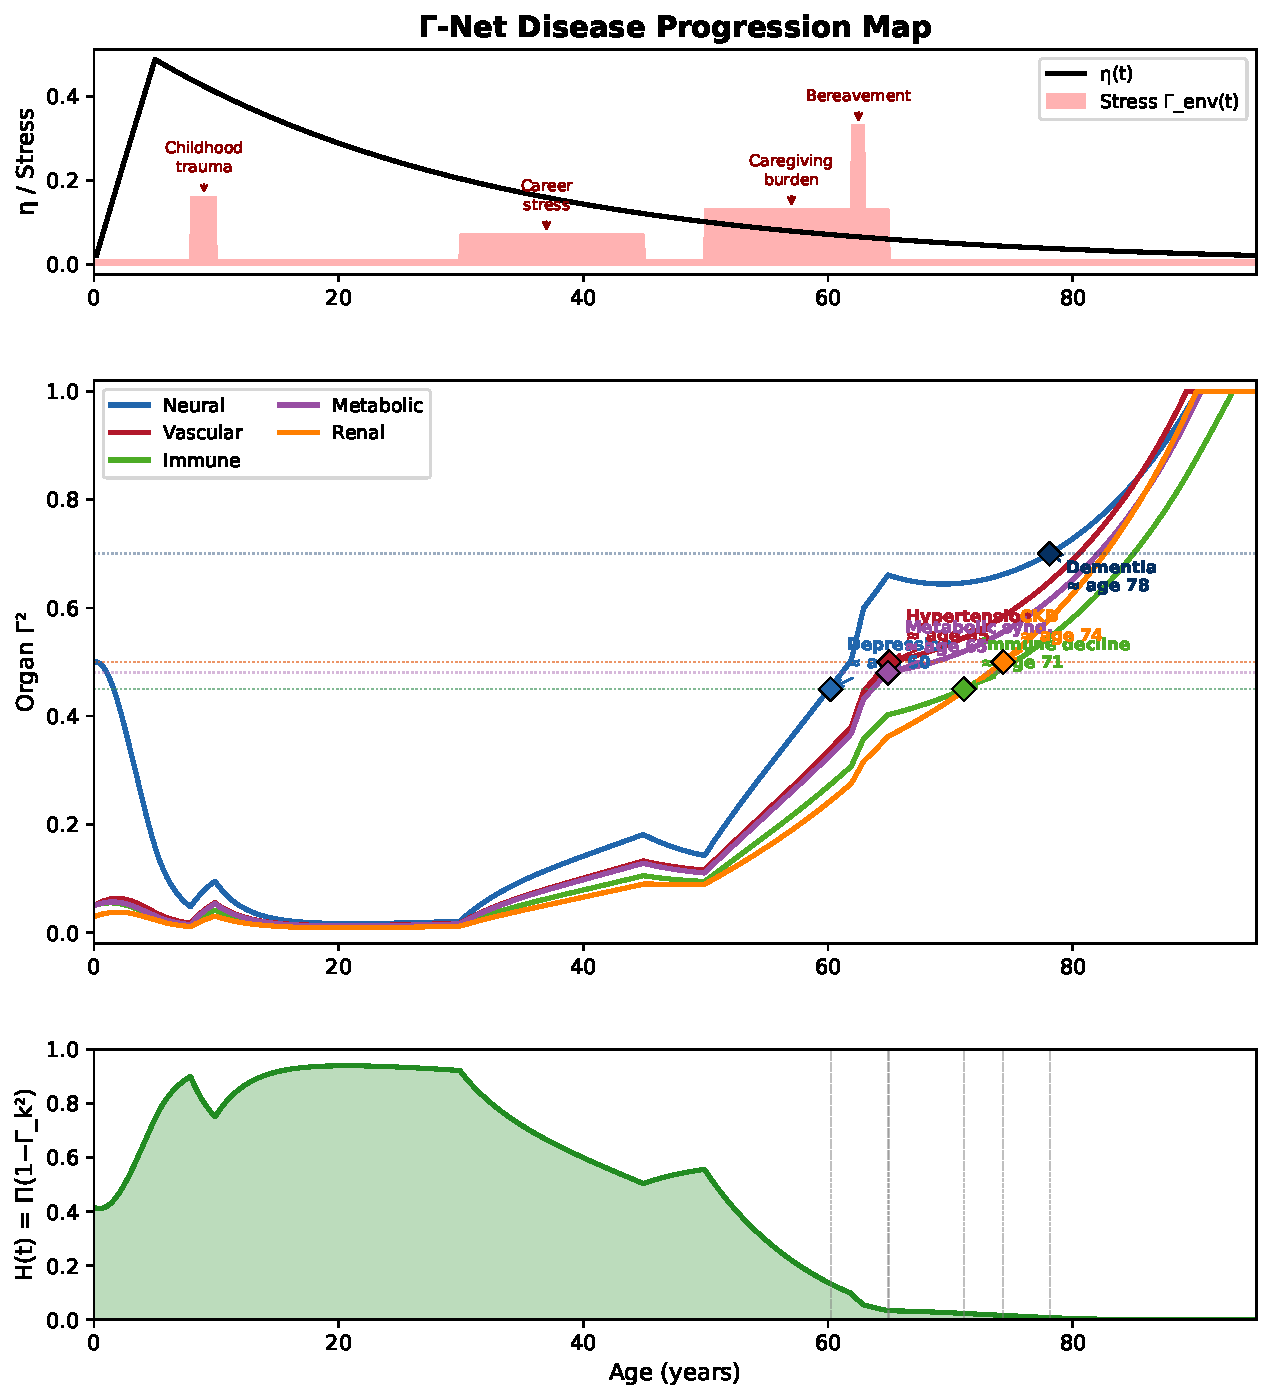
\includegraphics[width=\columnwidth]{../figures/fig_disease_progression.pdf}
  \caption{$\Gamma$-Net disease progression map for a
  representative high-risk trajectory.
  \textbf{Top}: homeostatic repair capacity $\eta(t)$ and
  external stress profile.
  \textbf{Middle}: five coupled organ $\Gamma^2$ trajectories;
  diamonds mark sustained threshold crossings (disease onset).
  \textbf{Bottom}: total health product
  $H(t) = \prod_k(1-\Gamma_k^2)$.
  All parameters are derived from Papers~2--3 physics;
  no curve fitting to clinical data.}
  \label{fig:disease-progression}
\end{figure}

\begin{remark}[Disease onset as impedance phase transition]
\label{rem:disease-phase-transition}
The positive-feedback term $\beta_k\,\Gamma_k^4$ in
Eq.~(\ref{eq:coupled-G2}) creates a saddle-node
bifurcation: below a critical forcing level,
$\Gamma_k^2$ remains at a low, stable equilibrium;
above it, no low-$\Gamma$ equilibrium exists and
the channel collapses toward $\Gamma_k^2 = 1$.
Disease onset is therefore not a gradual deterioration
but a \emph{phase transition}---the system crosses a
tipping point beyond which homeostatic repair cannot
restore the low-$\Gamma$ state.
The coupling matrix $C_{kj}$ then propagates this
collapse to downstream organs, explaining why
chronic diseases rarely appear in isolation.
\end{remark}


\subsection{Recovery dynamics: what happens when the
  stressor disappears}
\label{sec:recovery}

The preceding analysis raises the central clinical
question: if the external stressor is removed
($s(t) = 0$ for $t > t_{\text{off}}$),
does the system return to health?
Setting $s = 0$ in Eq.~(\ref{eq:coupled-G2}) gives
\begin{equation}
  \frac{d\Gamma_k^2}{dt}\bigg|_{s=0}
  = -\eta(t)\,\Gamma_k^2
    + \sum_{j \neq k} C_{kj}\,\Gamma_j^2
    + \beta_k\,\Gamma_k^4
    + \delta_k(t)\,.
  \label{eq:recovery}
\end{equation}
Recovery requires the repair term
$\eta\,\Gamma_k^2$ to dominate the sum of
inter-channel coupling, positive feedback, and
aging damage.
Three regimes emerge:

\begin{enumerate}
  \item \textbf{Pre-bifurcation (reversible).}
    If every channel satisfies
    $\Gamma_k^2 < \Gamma_k^{*2}$
    (below the saddle-node threshold of
    Remark~\ref{rem:disease-phase-transition}),
    then $\eta$ exceeds the combined
    $C_{kj}$ and $\beta_k$ terms, and
    $\Gamma_k^2 \to \Gamma_{k,\text{eq}}^{\text{low}}$
    exponentially.
    Clinically: acute stress, adjustment disorder,
    early burnout---symptoms resolve within weeks
    to months after stressor removal.

  \item \textbf{Post-bifurcation, single channel
    (partially reversible).}
    If one channel (typically neural) has crossed
    its bifurcation point
    $\Gamma_n^2 > \Gamma_n^{*2}$
    but the downstream channels have not,
    self-sustained positive feedback
    ($\beta_n\,\Gamma_n^4$) keeps the neural
    attractor locked even at $s = 0$.
    However, the coupling terms
    $C_{kn}\,\Gamma_n^2$ have not yet pushed
    other channels past their thresholds.
    Recovery requires \emph{active intervention}
    to lower $\Gamma_n^2$ below the
    bifurcation point---pharmacotherapy
    (modulate $\eta$, widen basin),
    psychotherapy (provide corrective C2
    gradient), or both
    (Paper~3, Sec.~XIV.B).
    Once $\Gamma_n^2$ is pulled below
    $\Gamma_n^{*2}$, the remaining channels
    self-heal via their intact $\eta$.
    Clinically: GAD, moderate PTSD, early
    depression---treatable but not
    self-resolving.

  \item \textbf{Post-bifurcation, multi-channel
    (structurally irreversible).}
    If the cascade has propagated through $C_{kj}$
    and two or more channels have independently
    crossed their bifurcation thresholds,
    each channel sustains the others even after
    the stressor is removed:
    \begin{equation}
      \eta\,\Gamma_k^2
      < \sum_{j \neq k} C_{kj}\,\Gamma_j^2
        + \beta_k\,\Gamma_k^4
      \quad \forall\; k \in \text{locked channels.}
      \label{eq:irreversible}
    \end{equation}
    No single-channel intervention suffices because
    lowering $\Gamma_k^2$ in one channel is
    immediately re-driven by the locked neighbours.
    Clinically: Complex PTSD with metabolic
    syndrome, chronic pain with depression and
    immune decline---the ``treatment-resistant''
    multimorbidity that consumes disproportionate
    healthcare resources.
    The only viable strategy is \emph{simultaneous
    multi-channel intervention}: e.g.\ combined
    psychotherapy (neural) + exercise
    (vascular--metabolic) + anti-inflammatory
    (immune), each targeting a different $\Gamma_k^2$
    below its respective bifurcation point.
\end{enumerate}

\begin{remark}[Why ``just removing the stress''
  is sometimes not enough]
\label{rem:hysteresis}
The saddle-node bifurcation in
Eq.~(\ref{eq:coupled-G2}) exhibits
\emph{hysteresis}: the stress level required to
\emph{trigger} the phase transition
($s_{\text{onset}}$) is lower than the stress
\emph{reduction} required to reverse it
($s_{\text{recovery}} < 0$, i.e.\ active repair
is needed).
In everyday language: ``the damage is done''
is not a metaphor but a statement about the
bifurcation diagram.
The gap between $s_{\text{onset}}$ and
$s_{\text{recovery}}$ widens with time spent in
the high-$\Gamma$ state, because aging damage
$\delta_k(t)$ continues to accumulate and
$\eta(t)$ continues to decline.
Early intervention---before the cascade crosses
a second channel's threshold---is therefore not
merely preferable but \emph{physically
qualitatively different} from late intervention.
\end{remark}

\noindent
The recovery hierarchy also predicts a
\emph{channel ordering} for rehabilitation:
the channel with the lowest
$\beta_k / \eta$ ratio recovers first when stress
is removed, while the channel with the highest
ratio is the last to unlock.
In the five-organ model, vascular $\Gamma_v^2$
typically has the fastest self-repair
(exercise increases $\eta_v$ directly via
shear-stress remodeling), while neural
$\Gamma_n^2$ is slowest
(structural $Z_s$ changes require months of
sustained C2 input).
This predicts a clinically testable
\emph{recovery sequence}: physical health
markers (blood pressure, HbA1c) improve before
psychological symptoms (mood, sleep, cognition)
---consistent with rehabilitation medicine
observations that metabolic improvement often
precedes and enables psychological recovery.


\subsection{Caregiver triple-load model}
\label{sec:triple-load}

Long-term caregivers experience three simultaneous
$\Gamma^2$-injection channels with no comparable
discharge path.  Their impedance-debt rate is:
\begin{equation}
  \frac{dD_Z}{dt}
  = \underbrace{\lambda\,\Gamma_{\text{other}}^2}_{\text{empathic load}}
  + \underbrace{\Gamma_{\text{moral}}^2}_{\text{moral constraint}}
  + \underbrace{\sigma\,s(t)}_{\text{daily stressor}}
  - \underbrace{\eta(t)\,\Gamma^2}_{\text{repair}}\,.
  \label{eq:triple-load}
\end{equation}

\emph{Channel~1: empathic load.}
$\Gamma_{\text{other}}^2$ is the care-recipient's
frozen mismatch (typically PTSD or dementia,
$\Gamma^2\!\approx\!1$).
The empathic coupling $\lambda>0$ injects this
energy into the caregiver's neural channel
every contact hour; it cannot be ``turned off'' without
severing the care relationship.

\emph{Channel~2: moral constraint.}
Social and internalised norms (``you must not give up'')
target the caregiver's fatigue pattern.
Because the caregiver's $\eta$ is already depleted,
this pattern is approaching or inside
$\mathcal{S}_{\text{eff}}$.
By the Moral Constraint Theorem
(Paper~4, Theorem~\ref{thm:moral-constraint}),
the demand injects $\Gamma_{\text{moral}}^2>0$
with $\Delta Z_{\text{corrective}}=0$---pure injury.

\emph{Channel~3: moral prohibition on $\lambda$-reduction.}
The only physically available knob for reducing
$dD_Z/dt$ is to lower $\lambda$ (set boundaries,
take breaks, delegate).
Moral pressure \emph{forbids} this adjustment
(``abandonment''), locking the intake valve open.

\begin{remark}[Structural inevitability of caregiver
disease]
\label{rem:caregiver-inevitable}
In Eq.~(\ref{eq:triple-load}), the first three terms
are approximately constant or increasing (the
care-recipient's $\Gamma^2$ does not spontaneously
decrease; moral pressure does not spontaneously relent;
daily stress persists).
The repair term $\eta(t)\,\Gamma^2$ decreases because
$\eta(t)$ declines by Arrhenius kinetics
and is further depressed by cortisol-mediated
hippocampal atrophy from the chronic load itself.
Therefore $dD_Z/dt > 0$ for all future time---the deficit
is \emph{structurally guaranteed} to widen.
The resulting disease cascade
(Eq.~\ref{eq:coupled-G2}, Fig.~\ref{fig:disease-progression})
is not a risk factor but a mathematical inevitability
unless institutional intervention (shift rotation,
$\lambda$-reduction protocols) is applied.
\end{remark}

\begin{remark}[Compassion fatigue, burnout, vicarious
trauma: one equation, three names]
\label{rem:fatigue-taxonomy}
Clinical nomenclature distinguishes compassion fatigue,
burnout, and vicarious trauma as separate syndromes.
Within Eq.~(\ref{eq:triple-load}) they are three
regimes of the same physics:
\begin{center}
\begin{tabular}{lll}
\toprule
Syndrome & Dominant term & $\mathcal{S}_{\text{eff}}$ status \\
\midrule
Burnout & $\sigma\,s(t)$ (workload) & not yet sealed \\
Compassion fatigue & $\lambda\,\Gamma_{\text{other}}^2$ &
  approaching seal \\
Vicarious trauma &
  $\lambda\,\Gamma_{\text{other}}^2$ sealed into
  $\mathcal{S}_{\text{eff}}$ & sealed \\
\bottomrule
\end{tabular}
\end{center}
The physical distinction is whether the dominant
$\Gamma^2$ pattern has entered $\mathcal{S}_{\text{eff}}$:
if not, rest and workload reduction suffice
(burnout); if sealed, only pharmacological $\eta$-elevation
plus guided C2 gradient (combined therapy) can rewrite
the pattern---identical to the PTSD treatment protocol
(Paper~3, Sec.~13b.2).
Rest alone cannot unseal the null space
(Second Law, Paper~4, Theorem~\ref{thm:second-law}).
\end{remark}

\subsection{Surface observability: skin as impedance boundary}
\label{sec:surface-readout}

Long-term caregivers and high-empathy individuals
sustain a chronic triple-load deficit
(Eq.~(\ref{eq:triple-load})).
When $dD_Z/dt > 0$ persists, the accumulated
impedance debt diffuses through the organ coupling
matrix $C_{kj}$:
%
\[
  \text{Neural}
  \;\xrightarrow{C_{21}}\;
  \text{Vascular}
  \;\xrightarrow{C_{42}}\;
  \text{Metabolic}
  \;\to\;
  \text{Surface}
\]
%
Neuralside $\Gamma_n^2$ elevation first disrupts
the hypothalamic--pituitary--adrenal (HPA) axis
and autonomic regulation, raising vascular
$\Gamma_v^2$; this in turn perturbs metabolic
and immune C2 networks, ultimately manifesting
as micro-circulatory and structural remodelling
in peripheral tissue---especially skin and hair
follicles.
Crucially, the cascade passes through a
\emph{neuroendocrine--behavioural intermediate layer}
before reaching the surface:
disrupted sleep architecture, appetite dysregulation,
irritability, and reduced exercise tolerance are all
observable consequences of HPA-axis $\Gamma^2$
overload that temporally precede overt skin changes.
The full observable chain is therefore
%
\[
  \underbrace{\text{Neural}\;\Gamma_n^2\!\uparrow}
    _{\text{mood, cognition}}
  \;\to\;
  \underbrace{\text{HPA / ANS}}
    _{\text{sleep, appetite, temper}}
  \;\to\;
  \underbrace{\text{Vascular}\;\Gamma_v^2\!\uparrow}
    _{\text{micro-circulation}}
  \;\to\;
  \underbrace{\text{Metabolic / Immune}}
    _{\text{collagen, inflammation}}
  \;\to\;
  \underbrace{\text{Surface}}
    _{\text{skin, hair}}
\]
%

\begin{remark}[Empathic overload as single-core
running dual-core load]
\label{rem:single-core}
The empath's $\Gamma$-network physically simulates
another person's pain state:
her own daily mismatch load $\sigma\,s(t)$ remains,
while the empathic channel adds
$\lambda\,\Gamma^2_{\text{other}}$---effectively
doubling the total $\Gamma^2$ input on a single
repair budget $\eta(t)$.
This is analogous to a single-core processor forced
to sustain a dual-core workload:
neither task can be suspended, thermal budget
($\eta$) is shared, and sustained over-clocking
leads to monotonic performance degradation.
The neuroendocrine--behavioural layer
(HPA dysregulation, sleep fragmentation,
affect lability) constitutes the first
externally observable ``thermal throttling''
of this overloaded system,
preceding the dermal readout by weeks to months.
\end{remark}

The critical observation is that skin is not an
isolated organ but the \emph{outermost boundary
condition} of the whole-body impedance network.
It simultaneously receives the output state of
vascular, metabolic, and immune channels,
making it a natural terminal load and
real-time readout:
%
\begin{center}
\begin{tabular}{lll}
\toprule
Internal $\Gamma^2$ channel & Skin manifestation &
  Colloquial term \\
\midrule
Vascular $\Gamma_v^2\!\uparrow$
  $\to$ micro-circulatory mismatch &
  Pallor, dark circles, dull complexion &
  ``Bad colour'' \\
Metabolic $\Gamma_{\text{met}}^2\!\uparrow$
  $\to$ collagen \& hydration imbalance &
  Roughness, sallowness, loss of elasticity &
  ``Poor skin quality'' \\
Immune $\Gamma_{\text{imm}}^2\!\uparrow$
  $\to$ inflammatory leakage &
  Redness, hypersensitivity, eczema flare-up &
  ``Skin deterioration'' \\
\bottomrule
\end{tabular}
\end{center}
%
A third party's intuitive visual assessment---``You
look worn out''---can therefore be re-read in the
$\Gamma$-language as a low-resolution impedance
tomography scan. The observer's cortex holds an
internal template
$Z_{\text{healthy}}$ (hue, luminance, uniformity);
when the observed surface impedance
$Z_{\text{obs}}$ deviates significantly, the visual
reflection coefficient
%
\begin{equation}
  \Gamma_{\text{visual}}
  = \frac{Z_{\text{obs}} - Z_{\text{healthy}}}
         {Z_{\text{obs}} + Z_{\text{healthy}}}
  \neq 0
  \label{eq:visual-gamma}
\end{equation}
%
is read out in higher cortical areas as
``something looks off.''

\begin{remark}[Detection threshold: null signal as
health certificate]
\label{rem:detection-threshold}
Equation~(\ref{eq:visual-gamma}) has an important
converse.
When diet, sleep, and stress are well regulated,
all three load terms in Eq.~(\ref{eq:triple-load})
remain small:
$\sigma\,s(t) \approx 0$,
$\lambda\,\Gamma^2_{\text{other}} \approx 0$,
$\Gamma^2_{\text{moral}} \approx 0$.
Hence $dD_Z/dt \lesssim 0$ and the repair capacity
$\eta(t)$ suffices to remodel daily mismatch back
to baseline.
Micro-circulation, collagen turnover, and immune
tone stay within normal fluctuation---the skin
terminal load is never pulled far from the
healthy template, so
$Z_{\text{obs}} \approx Z_{\text{healthy}}$
and $\Gamma_{\text{visual}} \approx 0$.
The observer's perceptual read-out is therefore
a \emph{null signal}: ``nothing looks wrong.''

This null signal is not an absence of information
but a positive measurement:
it certifies that all upstream $\Gamma^2$ channels
lie within the C2-repairable band.
Conversely, once any channel sustains
$\Gamma^2$ above the C2-repair ceiling---whether from
chronic stress ($\sigma\,s(t)$) or empathic overload
($\lambda\,\Gamma^2_{\text{other}}$)---the
surface deviation grows monotonically and the
observer transitions abruptly from null signal to
strong alarm (``this person has completely
deteriorated'').
The sharpness of this perceptual transition reflects
the threshold nonlinearity inherent in the
coupling cascade: sub-threshold $\Gamma^2$ is
invisible; supra-threshold $\Gamma^2$ is
unmistakable.
\end{remark}

\begin{remark}[Downstream convergence of empathic and
stress pathology]
\label{rem:downstream-convergence}
Empathic load ($\lambda\Gamma^2_{\text{other}}$ dominant)
and occupational stress ($\sigma\,s(t)$ dominant) differ
only in their \emph{upstream} input channel.
Once $\Gamma^2$ enters the coupling matrix $C_{kj}$,
the subsequent path
(Neural $\to$ Vascular $\to$ Metabolic $\to$ Surface)
is identical.
Consequently, from the skin's perspective as terminal
load they are branches of the same $\Gamma$-disease
tree (Sec.~\ref{sec:disease-progression}),
explaining why a caregiver who has tended a dementia
patient for years and an executive under chronic
workplace stress are visually indistinguishable
in their surface presentation.
\end{remark}

\subsection{Obesity as impedance-driven metabolic strategy}
\label{sec:obesity}

Conventional discourse frames obesity as a failure
of self-control.
The $\Gamma$-framework reveals a different causal
structure: chronic $\Gamma^2$ overload triggers a
whole-body metabolic reallocation that makes
overeating a \emph{physically rational} compensatory
strategy rather than a moral deficiency.

\paragraph{Selfish-brain cascade.}
Under sustained stress ($\sigma\,s(t)$ large) or
empathic overload
($\lambda\,\Gamma^2_{\text{other}}$ large),
cumulative impedance debt $D_Z$ rises and the neural
channel reads persistent supply instability.
The brain's response---well documented as the
``selfish brain'' hypothesis~\cite{Peters2011}---is
to up-regulate caloric intake, particularly
fast-availability substrates (sugar, fat),
and to down-regulate satiety sensitivity.
In the $\Gamma$-language:
%
\begin{equation}
  \text{High }\Gamma_n^2
  \;\xrightarrow{\text{HPA axis}}\;
  \text{insulin/glucose redistribution}
  \;\xrightarrow{\text{reward}}\;
  \text{appetite}\!\uparrow,\;
  \text{satiety sensitivity}\!\downarrow
  \label{eq:selfish-brain}
\end{equation}
%
The behavioural output---compulsive eating---is the
neural channel's attempt to stabilise its own $D_Z$
at the expense of the metabolic channel.

\paragraph{Leptin resistance as impedance mismatch.}
In sustained obesity, circulating leptin is high,
but the hypothalamic leptin-receptor pathway exhibits
reduced signal transmission~\cite{Moran2019}---a
textbook impedance mismatch.
The satiety signal $Z_{\text{leptin}}$ is present
at the source but cannot couple into the load
($Z_{\text{hypothalamus}}$), so the brain never
receives the ``fat stores are sufficient'' message.
Formally, the leptin channel's reflection coefficient
%
\[
  \Gamma_{\text{leptin}}
  = \frac{Z_{\text{hypothalamus}}
          - Z_{\text{leptin}}}
         {Z_{\text{hypothalamus}}
          + Z_{\text{leptin}}}
  \;\to\; 1
\]
%
approaches unity: the signal is almost totally
reflected, and the transmitted fraction
$T_{\text{leptin}} = 1 - \Gamma_{\text{leptin}}^2
\to 0$.
This is not a character flaw;
it is a hardware-level C2-pathway failure.

\paragraph{Hedonic eating as short-term
\texorpdfstring{$\Gamma^2$}{Gamma-squared} reduction.}
Ghrelin, leptin, and the mesolimbic reward circuit
jointly modulate both hunger and hedonic
valuation~\cite{Schellekens2012}.
High-calorie intake produces a transient subjective
$\Gamma^2$ reduction (``comfort''), trading a brief
mismatch relief for a larger long-term $D_Z$
increment (weight gain, insulin resistance,
cardiovascular load):
%
\[
  \underbrace{\Delta\Gamma^2_{\text{short}}
    < 0}_{\text{hedonic relief}}
  \;,\quad
  \underbrace{\Delta D_{Z,\text{long}}
    \gg 0}_{\text{metabolic debt}}
\]
%
This is the metabolic analogue of the PTSD
flashback--avoidance cycle (Paper~3):
a locally rational response that is globally
destructive.

\begin{remark}[Moral blame as secondary metabolic injury]
\label{rem:obesity-blame}
Applying the Moral Constraint Theorem
(Paper~4, Theorem~\ref{thm:moral-constraint})
to the obese individual:
the eating pattern is already approaching or inside
$\mathcal{S}_{\text{eff}}$
(sealed by years of reinforced reward circuitry),
so moral condemnation (``lack of self-discipline'')
injects $\Gamma^2_{\text{blame}}$ without any
corresponding $\Delta Z_{\text{corrective}}$.
The result is strictly additional impedance debt:
the subject now carries the original metabolic
$\Gamma^2$ \emph{plus} a shame/stigma $\Gamma^2$
that further activates the stress--appetite
cascade of Eq.~(\ref{eq:selfish-brain}),
accelerating the very pathology it purports to
correct.
Weight-stigma research confirms precisely this
paradox: moral pressure to lose weight predicts
\emph{increased} weight gain over
time~\cite{Sutin2015}.
\end{remark}

\begin{remark}[Positive-feedback closure:
obesity as mathematical attractor]
\label{rem:obesity-loop}
The metabolic cascade of
Eq.~(\ref{eq:selfish-brain}) is not a linear
chain but a \emph{closed positive-feedback loop}:
%
\[
  \text{Metabolic }\Gamma^2\!\uparrow
  \;\to\;
  \text{peripheral deterioration}
  \;\to\;
  \text{neural detection}
  \;\to\;
  \text{energy reallocation}
  \;\to\;
  \text{appetite}\!\uparrow
  \;\to\;
  \text{Metabolic }\Gamma^2\!\uparrow
\]
%
Each cycle amplifies the previous round's $\Gamma^2$.
As long as the environmental stress
$\sigma\,s(t)$ persists, the loop gain exceeds unity
and cumulative weight gain is not a lifestyle choice
but a \emph{fixed-point attractor} of the coupled
dynamics---obesity emerges as a mathematical
inevitability on physiological timescales.
\end{remark}

\begin{remark}[``Willpower'' as
$\eta_{\text{pfc}}(t)$: a depleting physical
quantity, not a moral virtue]
\label{rem:willpower}
What common discourse calls ``willpower'' or
``self-control'' corresponds, in the $\Gamma$-language,
to the prefrontal cortex's override capacity
over subcortical drive signals---i.e.\ the
prefrontal repair rate $\eta_{\text{pfc}}(t)$.
But the prefrontal cortex is itself a channel
within the same impedance network;
its $\eta_{\text{pfc}}(t)$ decays by the same
Arrhenius kinetics and is further depressed by
the chronic cortisol load generated by the
metabolic--stress cascade.
Therefore $\eta_{\text{pfc}}(t)$ is not a free
parameter that can be summoned at will;
it is a \emph{state variable} already depleted by
the very process it is asked to override:
%
\[
  \eta_{\text{pfc}}(t)
  = \eta_0 \, e^{-E_a/k_B T}
    \cdot f_{\text{cortisol}}(D_Z(t))
  \;\xrightarrow[\text{chronic }\Gamma^2]{}\;
  \text{depleted}
\]
%
Asking a chronically stressed or obese individual
to ``simply exercise self-control'' is therefore
not a moral appeal but a request to draw on
a resource that the physics has already consumed.
The illusion that willpower is a character trait
rather than a depletable physical budget arises
because, in low-$\Gamma^2$ individuals
(low stress, intact $\eta$), prefrontal override
appears effortless---just as a lightly loaded CPU
appears to have ``infinite patience.''
The concept dissolves once the load exceeds the
repair capacity, which is precisely the regime
in which it is most demanded.
\end{remark}

\begin{proposition}[Non-existence of free willpower:
proof by contradiction from psychiatric epidemiology]
\label{prop:no-free-will}
\emph{Claim.}\;
``Willpower'' is not a free parameter of the
human system.

\emph{Proof.}\;
Suppose, for contradiction, that willpower
were a freely available override---i.e.\ that
every agent possesses an unbounded
$\eta_{\text{pfc}}$ capable of suppressing
any $\Gamma^2$ pattern at any time.
Then no mismatch could persist against the agent's
intention:
every depressive episode could be willed away,
every compulsive behaviour halted, every anxiety
loop interrupted.
In other words, $\Gamma^2$ could never
accumulate to clinical threshold in any channel,
and \emph{no mental illness could exist}.

Empirically, approximately 970 million
people worldwide carry a diagnosed mental
disorder as of 2019 (WHO Global Burden of
Disease).
This is a direct contradiction.
Therefore the premise is false:
willpower is not a free parameter but a
state-dependent, depletable physical quantity
$\eta_{\text{pfc}}(t)$, subject to the same
Arrhenius decay, cortisol suppression, and
$\Gamma^2$-induced degradation as every other
channel in the impedance network.
$\square$
\end{proposition}

Paper~4~\cite{Paper4} refines this further:
even when $\eta_{\text{pfc}}$ is metabolically
adequate, effective willpower requires (i)~trained
thalamic gate speed ($Q_{\text{gate}}$) and
(ii)~a calibrated impedance map
($1 - \langle\Gamma^2_{\text{memory}}\rangle$);
the three factors compose multiplicatively
(Paper~4, Eq.~(14)~\cite{Paper4}),
so a single zero factor extinguishes volitional
capacity regardless of the other two.


\subsection{Immune--metabolic bidirectional feedback:
  the inflammation--insulin trap}
\label{sec:imm-met-loop}

Among the off-diagonal entries of the coupling matrix
$C_{kj}$ in Eq.~(\ref{eq:coupled-G2}), the pair
$(C_{\text{imm,met}},\,C_{\text{met,imm}})$ deserves
independent analysis because \emph{both} are positive
and mutually reinforcing, creating a local
positive-feedback sub-system even when
the remaining channels are stable.

Write the two-channel subsystem:
\begin{align}
  \frac{d\Gamma_{\text{imm}}^2}{dt}
  &= -\eta\,\Gamma_{\text{imm}}^2
     + C_{\text{imm,met}}\,\Gamma_{\text{met}}^2
     + \beta_{\text{imm}}\,\Gamma_{\text{imm}}^4\,,
  \label{eq:imm-loop} \\
  \frac{d\Gamma_{\text{met}}^2}{dt}
  &= -\eta\,\Gamma_{\text{met}}^2
     + C_{\text{met,imm}}\,\Gamma_{\text{imm}}^2
     + \beta_{\text{met}}\,\Gamma_{\text{met}}^4\,.
  \label{eq:met-loop}
\end{align}
The mutual-excitation terms form a closed cycle:
adipocyte hypertrophy raises metabolic $\Gamma_{\text{met}}^2$
(insulin resistance, hepatic lipogenesis); this triggers
macrophage infiltration and pro-inflammatory cytokine
release (IL-6, TNF-$\alpha$), raising immune
$\Gamma_{\text{imm}}^2$ (chronic low-grade inflammation,
elevated CRP); the inflammatory milieu further impairs
insulin receptor signalling, pushing
$\Gamma_{\text{met}}^2$ higher still:
\[
  \Gamma_{\text{met}}^2\!\uparrow
  \;\xrightarrow{C_{\text{imm,met}}}
  \;\Gamma_{\text{imm}}^2\!\uparrow
  \;\xrightarrow{C_{\text{met,imm}}}
  \;\Gamma_{\text{met}}^2\!\uparrow
  \;\to\;\cdots
\]

Linearising about a small perturbation
$\delta\Gamma_k^2$ around equilibrium,
the Jacobian of the subsystem has eigenvalues
\begin{equation}
  \lambda_\pm
  = -\eta + \tfrac{1}{2}
    \bigl(\alpha_{\text{imm}} + \alpha_{\text{met}}\bigr)
  \pm \sqrt{C_{\text{imm,met}}\,C_{\text{met,imm}}
    + \tfrac{1}{4}(\alpha_{\text{imm}} - \alpha_{\text{met}})^2}\,,
  \label{eq:imm-met-eigenvalue}
\end{equation}
where
$\alpha_k \equiv 2\beta_k\,\Gamma_{k,\text{eq}}^2$.
The subsystem destabilises when $\lambda_+ > 0$, i.e.
\begin{equation}
  \sqrt{C_{\text{imm,met}}\,C_{\text{met,imm}}}
  > \eta - \tfrac{1}{2}
    (\alpha_{\text{imm}} + \alpha_{\text{met}})\,.
  \label{eq:imm-met-threshold}
\end{equation}
This is the \emph{inflammation--insulin trap}:
once the geometric mean of the mutual coupling
exceeds the net repair margin, the two channels
lock into a self-sustaining high-$\Gamma^2$
fixed point---metabolic syndrome with chronic
inflammation---even if the original neural stressor
has been removed.

Clinical correlates are well documented:
obesity $\to$ elevated CRP $\to$ type~2 diabetes
$\to$ further weight gain constitutes the
``metabolic--inflammatory'' comorbidity cluster
(\emph{coupled-subsystem divergence} in $\Gamma$
language: two channels simultaneously locked
above their respective $\theta$).
In recovery-dynamics terms
(Sec.~\ref{sec:recovery}), this sub-loop can
achieve regime~3 (structurally irreversible)
\emph{independently} of the neural channel,
explaining why bariatric surgery
(which mechanically breaks the metabolic
$\beta_{\text{met}}\,\Gamma^4$ term)
can resolve both diabetes \emph{and} systemic
inflammation simultaneously---a dual-channel
reset that diet alone, targeting only
$\Gamma_{\text{met}}^2$, often cannot achieve.


\subsection{Acute versus chronic stress:
  bifurcation threshold under time-limited forcing}
\label{sec:acute-chronic}

The stress-injection term $\sigma_k\,s(t)$ in
Eq.~(\ref{eq:coupled-G2}) does not distinguish
beneficial from harmful stress; the distinction
emerges from the \emph{temporal integral} relative
to the repair term.

Consider a square-pulse stressor of amplitude $A$
and duration $\Delta t$:
\begin{equation}
  s(t) = A\,\bigl[\Theta(t) - \Theta(t - \Delta t)\bigr]\,,
  \label{eq:pulse-stress}
\end{equation}
where $\Theta$ is the Heaviside step.
During the pulse, the channel trajectories satisfy
\begin{equation}
  \Gamma_k^2(t) \approx \Gamma_{k,\text{eq}}
  + \frac{\sigma_k\,A}{\eta}
    \bigl(1 - e^{-\eta\,t}\bigr)\,,
  \label{eq:acute-response}
\end{equation}
to first order (neglecting $\beta_k$ and $C_{kj}$
for short pulses).
The peak excursion is bounded by
$\Delta\Gamma_k^2 \leq \sigma_k A / \eta$,
and after the pulse ends, $\eta$ drives the system
back exponentially with time constant $1/\eta$.
The system remains safe (regime~1 of
Sec.~\ref{sec:recovery}) provided
\begin{equation}
  \Gamma_{k,\text{eq}} + \frac{\sigma_k\,A}{\eta}
  < \Gamma_k^{*2}
  \quad (\text{bifurcation threshold})\,.
  \label{eq:safe-acute}
\end{equation}
This is the physics of \emph{beneficial acute stress}:
high-intensity exercise ($A$ large, $\Delta t$ small),
cold-water immersion, intermittent fasting---all push
$\Gamma_k^2$ transiently upward, stimulating C2 repair
(``hormesis''), and the system returns to baseline
before coupling or positive feedback can engage.

Contrast this with chronic stress:
$s(t) = a$ (constant, $a < A$) for $t \gg 1/\eta$.
The steady-state solution of
Eq.~(\ref{eq:coupled-G2}) now includes coupling:
\begin{equation}
  \Gamma_{k,\text{ss}}^2
  = \frac{\sigma_k\,a + \sum_j C_{kj}\,\Gamma_{j,\text{ss}}^2
         + \delta_k}
        {\eta - \beta_k\,\Gamma_{k,\text{ss}}^2}\,.
  \label{eq:chronic-ss}
\end{equation}
Even for small $a$, the denominator shrinks as
$\Gamma_{k,\text{ss}}^2$ rises
(positive feedback $\beta_k$), and the coupling
terms $C_{kj}$ inject additional load from
neighbouring channels.
The saddle-node bifurcation occurs at
\begin{equation}
  \eta = \beta_k\,\Gamma_k^{*2}
         + \frac{\partial}{\partial\Gamma_k^2}
           \sum_j C_{kj}\,\Gamma_j^2\,,
  \label{eq:chronic-bifurcation}
\end{equation}
a threshold that \emph{decreases} with age
(because $\eta(t)$ declines by Arrhenius kinetics
while $\delta_k(t)$ grows).

\begin{remark}[The exercise paradox resolved]
\label{rem:exercise}
Exercise is simultaneously a high-$\Gamma^2$
perturbation (muscles, cardiovascular) and the
most effective known intervention against chronic
disease.
The paradox dissolves once time scale is explicit:
exercise is \emph{acute} forcing
($\Delta t \sim 1$\,hour, then $s \to 0$)
that never reaches the bifurcation threshold
(Eq.~\ref{eq:safe-acute}), while the transient
$\Gamma^2$ elevation \emph{stimulates}
C2 remodeling---raising effective $\eta$ in
vascular and metabolic channels
(shear-stress--mediated endothelial adaptation,
mitochondrial biogenesis).
Chronic sedentary stress, by contrast, is
low-amplitude but \emph{never turns off}:
the system drifts toward the chronic steady state
(Eq.~\ref{eq:chronic-ss}) and eventually crosses
the bifurcation.
Exercise is therapeutic precisely because it is
\emph{intermittent and bounded}.
\end{remark}


% ============================================================
%  E0 EMERGENCE: DISEASE FROM TOPOLOGY ALONE
% ============================================================
\section{E0 Emergence: Disease from Topology Alone}
\label{sec:e0-emergence}

The twenty-nine $\Gamma$-networks (Table~\ref{tab:twentynine})
and the central controllers establish C2 universality
in the \emph{scalar} domain (one impedance channel per tissue).
A stronger claim follows: clinical pathology should
\emph{emerge} from the \emph{multi-dimensional} topology
of the $\Gamma$-network without any disease-specific code.

We define three emergence levels:
\begin{itemize}
  \item \textbf{E0 (True Emergence)}: only C1/C2/C3 + initial
    conditions.  Zero disease-specific flags, thresholds, or formulas.
  \item \textbf{E1 (Parameterised)}: C2 via
    \texttt{ImpedanceChannel.remodel()} with per-disease
    parameters ($Z_{\text{coeff}}$, severity).
  \item \textbf{E2 (Scripted)}: ad-hoc $Z$ updates.
    Legacy only; forbidden for new code.
\end{itemize}

\noindent
E0 is the gold standard: ``if you need a flag, it didn't
emerge.''
We test this with 29~tissue blueprints (\texttt{GammaTopology}
instances with biologically assigned \texttt{TissueType} and
mode count~$K$; Paper~0~\cite{Paper0}, Table~4)
and pure perturbations of initial conditions.
Detailed disease-emergence experiments are shown below for
the cardiovascular (11~nodes) and neural (9~nodes) systems;
all remaining 27~blueprints pass the same C1/C2 physics
verification (245~parametrised tests, 100\% pass).

\subsection{Cardiovascular E0: hypertension, MI, aortic stenosis}

Starting from a healthy 11-node cardiovascular
\texttt{GammaTopology} ($K \in \{4, 2, 1\}$;
Paper~1~\cite{Paper1}, Sec.~4.5):

\begin{enumerate}
  \item \textbf{Hypertension}: arteriolar $Z \times 2.0$
    $\Rightarrow$ $\Gamma^2$ at aorta$\to$arterioles
    increases; downstream capillary transmission decreases;
    C2 partially compensates over 300~ticks
    (remodeling = physiological adaptation).
  \item \textbf{Myocardial infarction}: sever
    aorta$\to$coronary edge
    $\Rightarrow$ coronary node isolated;
    total transmission decreases; topology is structurally
    different from HTN (correlation $< 0.99$).
  \item \textbf{Aortic stenosis}: valve $Z \times 3.0$
    $\Rightarrow$ LV-to-aorta $\Gamma^2$ increases
    (obstruction physics).
  \item \textbf{Dose--response}: arteriolar $Z$-factor
    $\{1.0, 1.5, 2.0, 3.0\}$ yields monotonically
    increasing $\Gamma^2$---severity scales with perturbation
    magnitude.
\end{enumerate}

\noindent
Thirteen automated tests
(\texttt{tests/test\_e0\_cardiovascular.py}), 100\% pass.
No disease model was coded; pathology identity is
determined solely by the perturbation type
(impedance shift vs.\ edge removal) and magnitude.

\subsection{Neural E0: ALS, stroke, PTSD, phantom pain}

Starting from a healthy 9-node neural
\texttt{GammaTopology} ($K \in \{5, 3, 2, 1\}$;
Paper~1~\cite{Paper1}, Sec.~4.6):

\begin{enumerate}
  \item \textbf{ALS} (motor neuron $Z \times 3.0$):
    $\Gamma^2$ at spinal$\to$motor edge increases;
    cumulative $\Aimp$ over 30~ticks is $2.9\times$ healthy;
    C2 partially compensates (plasticity).
  \item \textbf{Stroke} (cortex$\to$thalamus edge severed):
    descending motor transmission interrupted; ascending
    sensory pathway spared (different edges)---the deficit
    pattern is topologically determined.
  \item \textbf{PTSD} (nociceptor C driven at $5\times$
    normal amplitude for 100~ticks, then stopped):
    pain-pathway $\Gamma^2$ is altered during trauma
    \emph{and} a residual mismatch persists after stimulus
    removal---the physical basis of ``flashback'' as
    impedance echo.
  \item \textbf{Phantom limb pain}
    (motor neuron$\to$nociceptor edge severed):
    efferent modulation lost; nociceptor $\Gamma^2$ altered;
    ascending pain pathway remains intact---phantom
    ``sensation'' has a physical substrate
    (open-circuit reflection).
\end{enumerate}

\noindent
Seventeen automated tests
(\texttt{tests/test\_e0\_neural.py}), 100\% pass.
Additional tests verify:
\begin{itemize}
  \item ALS vs.\ stroke produce distinguishable
    $\Gamma$-trajectories (correlation $< 0.99$).
  \item Severity dose--response is monotonic (early ticks,
    before C2 convergence).
  \item $\Acut > 0$ at all times (irreducibility,
    $K{=}5 \to 3 \to 2 \to 1$).
  \item $\Acut$ remains $> 0$ after 300~ticks of C2 evolution
    (irreducible, not learnable).
  \item $\Aimp$ decreases under C2 (learnable).
  \item Neural $\Acut \geq$ cardiovascular $\Acut \times 0.5$
    (more $K$-level transitions $\Rightarrow$ higher
    geometric cost).
\end{itemize}

\subsection{Implications}

The 275 E0 tests (245~parametrised blueprint tests +
13~cardiovascular + 17~neural disease tests)
across all 29~organ-system topologies prove
that clinical pathology \emph{can} emerge from pure
impedance physics---C1/C2/C3 plus initial conditions---on
biologically realistic tissue topologies.
No disease-specific code, no flags, no thresholds,
no scoring systems.
The disease \emph{is} the perturbation; the clinical
pattern \emph{is} the resulting $\Gamma$-distribution.

\subsection{Thermal loop collapse: hypothermia and hyperthermia}
\label{sec:thermal-collapse}

Paper~3~\cite{Paper3} derives the $\Gamma^2\!\leftrightarrow\!T$
self-consistent loop: impedance mismatch produces heat,
heat maintains temperature, temperature sets viscosity
and repair rate, which in turn set $\Gamma$.
The 37$\,^\circ$C operating point is the stable fixed
point of this loop.  When the loop is driven outside its
basin of attraction, two E0 pathologies emerge---requiring
no disease-specific code:

\begin{center}
\begin{tabular}{@{}lll@{}}
\toprule
& \textbf{Hypothermia} & \textbf{Hyperthermia} \\
\midrule
Direction & $T \ll T^*$ & $T \gg T^*$ \\
Primary driver & $\eta(T)\!\uparrow$\,(viscosity) & $k_BT\!\uparrow$\,(noise) \\
$\Gamma$ mechanism & $Z_{\mathrm{bus}}\!\uparrow \to \Gamma^2\!\uparrow$ & $\delta\Gamma/\Gamma \propto K^{3/2}\delta T/T$ \\
First failure & Global $\Gamma^2$ rise & PFC ($K{=}5$) first \\
Clinical sign & Bradycardia $\to$ coma & Delirium $\to$ seizure \\
Feedback & Positive (less heat $\to$ colder) & Positive (more noise $\to$ more $\Gamma^2$) \\
C2 repair & Slowed (Arrhenius $\downarrow$) & Overwhelmed (noise $>$ signal) \\
\bottomrule
\end{tabular}
\end{center}

\noindent
Both are \textbf{E0}: they arise from C1/C2/C3 plus the
Arrhenius temperature dependence of $Z_{\mathrm{bus}}$
and $\eta_{\mathrm{learn}}$---no pathology-specific
parameters.  The clinical asymmetry (hypothermia is
global; hyperthermia hits PFC first) is a direct
consequence of the $K^{3/2}$ thermal vulnerability
derived in Paper~4~\cite{Paper4}.

This does not mean all 117~disease models in the codebase
are E0 today---most remain E1 (15) or legacy E2 (102).
But the existence proof changes the target:
E0 is achievable, and every E2 model is a candidate for
elimination via topology-based emergence.


\subsection{Sleep disorders as gate-leak pathology}
\label{sec:sleep-disorders}

Paper~3~\cite{Paper3} derives the gate-leak inequality:
\begin{equation}
  G_i^2\;\Gamma_i^2\;P_{\mathrm{in},i}
  \;>\;
  4\,k_B T\,R_{\mathrm{eff}}\,\Delta f
  \;\equiv\; P_\theta
  \tag{P3, Eq.\,10}
\end{equation}
as the physical condition for forced awakening.
Three clinically distinct sleep disorders map onto
three different structural failures within this
single inequality:

\paragraph{Insomnia: $\Gamma_i^2$ overload.}
Chronic stress or trauma forges one or more channels
at high structural mismatch ($\Gamma_i^2 \gg
\langle\Gamma^2\rangle$).
The thalamic gate~$G_i$ is at its physical minimum,
yet the leaked power still exceeds~$P_\theta$.
Clinical consequence: the patient ``cannot fall asleep''
despite exhaustion.
The standard epidemiological correlates---anxiety,
rumination, chronic pain---are precisely the conditions
that elevate $\Gamma_i^2$ on specific channels.
Pharmacological intervention (e.g.\ benzodiazepines)
temporarily increases gate attenuation (lowers~$G_i$);
durable resolution requires C2 remodelling of the
underlying $\Gamma_i^2$
(cognitive-behavioural therapy for insomnia, CBT-I,
provides the sustained counter-signal).

\paragraph{Narcolepsy: $Z_{\mathrm{anchor}}$ loss.}
The orexin (hypocretin) system provides the structural
anchor $Z_{\mathrm{anchor}}$ that prevents
$Z_{\mathrm{arousal}}$ from drifting below the
consciousness threshold.
Autoimmune destruction of orexin neurons
(type-1 narcolepsy) eliminates this anchor;
$Z_{\mathrm{arousal}}$ becomes a random walk
that crosses threshold at unpredictable intervals
$\to$ sleep attacks.
Cataplexy---the sudden loss of muscle tone during
strong emotion---is the motor-gate analogue:
a limbic $\Gamma^2$ spike leaks through the
descending motor gate ($G_{\text{motor}} \to 0$),
the same gate-leak equation applied to the
efferent rather than afferent pathway.
Orexin receptor agonists (suvorexant class, inverse;
future orexin-2 agonists for narcolepsy) directly
target~$Z_{\mathrm{anchor}}$.

\paragraph{Hypersomnia: $\beta_{\mathrm{recal}}$ deficit.}
Idiopathic hypersomnia (IH) preserves the arousal
anchor but has a structurally low NREM recalibration
rate~$\beta_{\mathrm{recal}}$.
Impedance debt~$D_Z$ is never fully discharged
during sleep;
the organism requires abnormally long sleep times
and wakes with ``sleep inertia'' (residual~$D_Z$).
During the day, elevated baseline~$\langle\Gamma^2\rangle$
means the gate-leak condition barely holds:
any small increase in $P_{\mathrm{in}}$
(warm room, monotonous task) tips a channel past
$P_\theta$ and the system collapses back into sleep
$\to$ excessive daytime sleepiness.
Wake-promoting agents (modafinil, solriamfetol)
reduce the effective $D_Z$ load by increasing
$P_{\mathrm{in}}$ uniformly across channels,
keeping $G_i^2\,\Gamma_i^2\,P_{\mathrm{in}}$
above the ``awake'' operating regime.

\paragraph{Unified diagnostic map.}

\begin{center}
\begin{tabular}{@{}llll@{}}
\hline
\textbf{Disorder} & \textbf{Broken parameter}
  & \textbf{Gate-leak status}
  & \textbf{Treatment target} \\
\hline
Insomnia
  & $\Gamma_i^2$ too high
  & Cannot close (leak $> P_\theta$)
  & Lower $\Gamma_i^2$ (CBT-I, C2) \\
Narcolepsy
  & $Z_{\text{anchor}} \to 0$
  & Collapses suddenly
  & Restore anchor (orexin agonist) \\
Hypersomnia
  & $\beta_{\text{recal}}$ low
  & Barely holding
  & Raise $\beta_{\text{recal}}$ or $P_{\text{in}}$ \\
\hline
\end{tabular}
\end{center}

\noindent
All three disorders are \emph{structural} impedance
failures---each specifying a different physical
parameter---unified under a single gate-leak equation.
The clinical fact that insomnia and hypersomnia
often coexist (``tired but wired'') maps naturally
to a system where $\beta_{\text{recal}}$ is low
(undischarged $D_Z$) \emph{and} one channel has
high $\Gamma_i^2$ (chronic leak):
the patient is simultaneously too depleted to stay
awake and too activated to fall asleep.


% ============================================================
%  SECTION 10 — NHANES NETWORK PROPAGATION
% ============================================================
\section{Empirical Evidence: Network Propagation}
\label{sec:propagation}

This paper (Section~\ref{sec:nhanes}) validated $\Gamma$
within single organ systems.
Here we test a stronger prediction: adding a physical
measurement to one $\Gamma$-network should improve
predictions in \emph{coupled} networks through
impedance propagation at inter-network interfaces.

\subsection{Experimental design}

Using NHANES 1999--2018 (10~cycles, $n = 49{,}774$,
$7{,}770$ deaths, up to 20-year follow-up), four
configurations:
\begin{itemize}
  \item[A] Laboratory values only (27 items $\to$ 12 organs)
  \item[B] Labs + blood pressure (SBP, DBP, pulse pressure
    $\to$ vascular, cardiac, renal, neurological $Z$)
  \item[C] Labs + smoking status
    ($\to$ pulmonary, vascular, immune $Z$)
  \item[D] Full physics (Labs + BP + smoking)
\end{itemize}
All mappings use textbook reference intervals.
\textbf{Zero parameters are fitted to any outcome data.}

\subsection{Results}

\begin{table}[h]
\centering
\caption{All-cause mortality AUC by configuration.}
\label{tab:allcause}
\begin{tabular}{lcc}
\toprule
Configuration & AUC (95\% CI) & $\Delta$ vs.\ A \\
\midrule
A: Labs only    & 0.629 [0.622--0.636] & --- \\
B: Labs + BP    & 0.705 [0.699--0.711] & $+0.075$ \\
C: Labs + Smoke & 0.627 [0.620--0.634] & $-0.002$ \\
D: Full physics & 0.704 [0.698--0.710] & $+0.075$ \\
\bottomrule
\end{tabular}
\end{table}

\begin{table}[h]
\centering
\caption{Organ-specific death AUC: Labs (A) vs.\
Labs+BP (B).  ``Network'' organs receive no direct BP
input; improvement comes from inter-network $\Gamma$-coupling.}
\label{tab:propagation}
\begin{tabular}{lcccc}
\toprule
Organ & Type & AUC (A) & AUC (B) & $\Delta$ \\
\midrule
Cardiac   & Network & 0.508 & 0.674 & $+0.166$ \\
Neuro     & Network & 0.516 & 0.577 & $+0.061$ \\
Renal     & Network & 0.677 & 0.700 & $+0.024$ \\
Endocrine & Control & 0.814 & 0.814 & $+0.000$ \\
\bottomrule
\end{tabular}
\end{table}

\textbf{Cardiac death AUC improves from 0.508 (chance) to
0.674}---$\Delta = +0.166$---from a vascular measurement,
not a cardiac measurement.
SBP physically propagates through the vascular--cardiac
interface (afterload), so vascular $Z$ directly determines
cardiac $Z$.

Endocrine serves as a negative control: no significant
vascular--endocrine pressure interface exists, and
AUC is unchanged ($\Delta = 0.000$).

\textbf{This cross-organ improvement is the empirical
signature of network propagation.}

\begin{figure}[h]
  \centering
  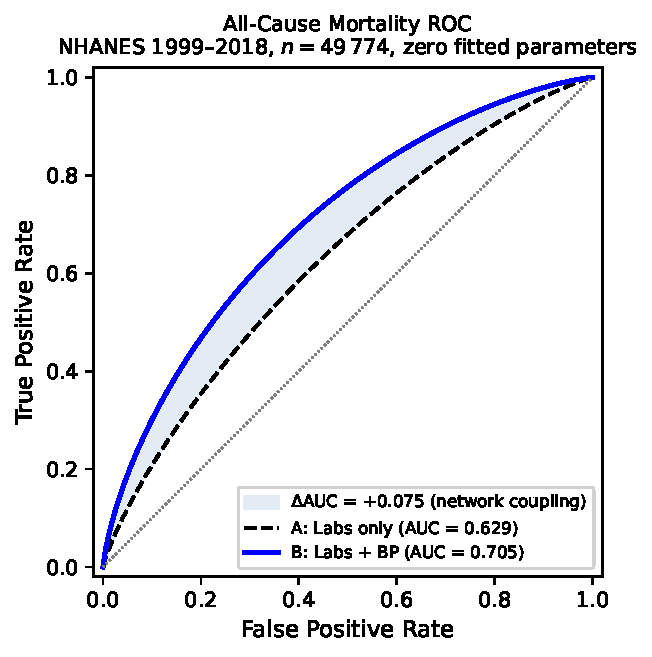
\includegraphics[width=\columnwidth]{../figures/roc_network_propagation.pdf}
  \caption{ROC curves for all-cause mortality:
  Configuration~A (labs only, AUC~$= 0.629$) vs.\
  Configuration~B (labs + BP, AUC~$= 0.705$).
  The shaded region represents the AUC gain from
  inter-network $\Gamma$-coupling through a single
  vascular measurement.}
  \label{fig:roc}
\end{figure}

\begin{figure}[h]
  \centering
  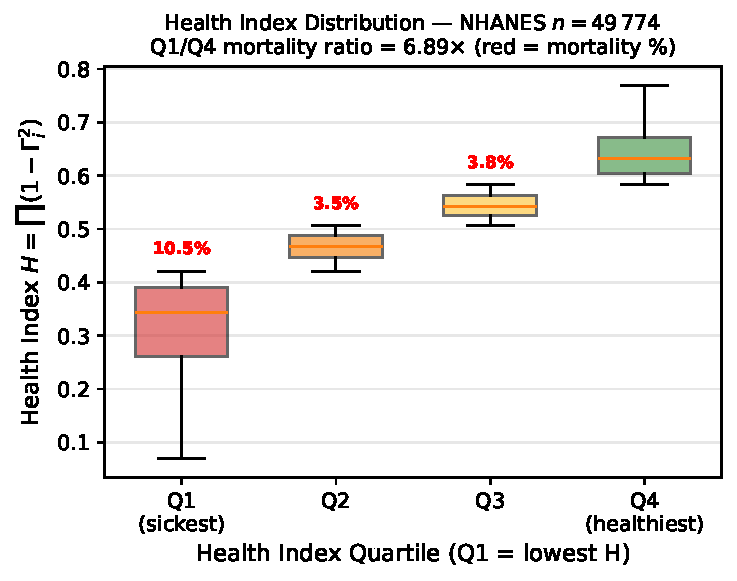
\includegraphics[width=\columnwidth]{../figures/health_index_boxplot.pdf}
  \caption{Health Index $H = \prod(1-\Gamma_i^2)$ by
  mortality quartile.  Q1 (sickest): median $H = 0.71$;
  Q4 (healthiest): median $H = 0.89$.
  Relative risk Q1/Q4 $= 6.89\times$.}
  \label{fig:boxplot}
\end{figure}


% ============================================================
%  SECTION 11 — PHYSICAL UNIQUENESS OF C2
% ============================================================
\section{Mathematical Uniqueness of C2}
\label{sec:c2-unique}

The gradient-descent derivation shows that C2 is the
\emph{unique} first-order update rule minimising reflected
energy at any repeatedly stimulated interface.
This is a mathematical theorem about gradient descent
on $\mathcal{A}[\Gamma]$, not a biological claim.

\subsection{The tissue is not the algorithm}

The remodeling machinery differs vastly: NMDA receptors
(neural), RANKL/OPG (bone), eNOS (vascular),
AID somatic hypermutation (immune), keratinocyte Ca$^{2+}$
(skin), HGF (liver), EPO (marrow), FSH receptors
(reproductive)---ten completely different molecular
machineries implementing the same equation.
The substrate determines the material constants
($\eta$, $Z_0$); the equation is dictated by physics.
That multiple unrelated machineries converge on the
same rule is \emph{consistent with} C2 being a
physical attractor; it is not evidence for any
particular evolutionary narrative.

\subsection{Objective function for viability}

The $\Gamma$-framework supplies a \emph{physical}
objective function:
\begin{equation}
  \mathcal{A} = \int_0^T \sum_i \Gamma_i^2(t)\,
  P_{\text{in},i}(t)\,dt\,.
\end{equation}
Any system whose $\mathcal{A}$ exceeds the
thermodynamic viability bound is physically excluded.
This is a constraint on what \emph{can} exist, not
an explanation of what \emph{does} exist.

\subsection{Sex as a boundary condition}

Sex does not alter C1--C3.  The hypothalamic--pituitary--gonadal
(HPG) axis sets sex-specific $Z_{\text{setpoint}}$ values:
testosterone raises $\eta_{\text{muscle}}$;
oestrogen modulates $Z_{\text{adipose}}$ and $Z_{\text{bone}}$
(menopause $\equiv Z_{\text{bone}} \uparrow,
\Gamma_{\text{bone}} \uparrow$);
pre-menopausal oestrogen maintains lower
$\Gamma_{\text{vasc}}$ via enhanced endothelial C2.
Sex is a parametric shift in initial and boundary
conditions, not a different dynamical law.


% ============================================================
%  SECTION 12 — FALSIFIABLE PREDICTIONS
% ============================================================
\section{Falsifiable Predictions}
\label{sec:predictions}

\begin{enumerate}
  \item \textbf{Cross-organ propagation (confirmed).}
    Adding SBP improves cardiac ($+0.166$), neuro ($+0.061$),
    renal ($+0.024$) AUC through network coupling.
    $\checkmark$

  \item \textbf{Control-organ invariance (confirmed).}
    Endocrine AUC unchanged when SBP added
    ($\Delta = 0.000$). $\checkmark$

  \item \textbf{Specialised biomarker upgrade.}
    Adding troponin/BNP (cardiac $Z$), liver elastography
    (hepatic $Z$), and spirometry (pulmonary $Z$) to
    the NHANES panel should raise organ-specific AUC
    substantially above current levels.

  \item \textbf{Microgravity bone loss follows C2 with
    $x_{\text{in}} = 0$.}
    Bone density loss rate in microgravity should be
    predictable from $\eta$ and pre-flight
    $\Gamma_{\text{mech}}$ without fitted parameters.

  \item \textbf{Vaccine booster spacing optimises
    $\sum x_{\text{in}} \cdot x_{\text{out}}$.}
    Optimal booster interval matches the time at which
    memory B-cell $x_{\text{out}}$ is maximally
    available but $\Gamma_{\text{immune}}$ has not
    fully decayed.

  \item \textbf{Adding FEV1/SpO$_2$ (pulmonary $Z$)
    will improve immune death AUC}
    through the pulmonary--immune interface.

  \item \textbf{Cross-modal impedance validation.}
    Organ impedances from blood biochemistry (Lab-$\Gamma$)
    should correlate with independently measured physical
    impedances (BIA, shear-wave elastography, pulse-wave
    velocity), closing every arrow in the
    chemistry$\to$structure$\to$impedance$\to\Gamma$ chain.

  \item \textbf{Prospective cohort.}
    Tracking $H = \prod(1-\Gamma_i^2)$ longitudinally
    should predict incident disease.

  \item \textbf{Skill-decay anti-chronology.}
    In longitudinal cohorts with detailed skill histories
    (age of acquisition), the order of functional loss
    under neurodegeneration should \emph{invert} the order
    of acquisition: skills acquired during the $\eta$-peak
    developmental window (native language, childhood motor
    sequences) will be the last to fail, while
    later-acquired skills (adult-onset second languages,
    midlife procedural skills) will fail earlier at matched
    structural-lesion burden.
    This follows from $\Delta Z_s \propto
    \int \eta(\tau)\,\Gamma_s\,x_{\text{in}}
    x_{\text{out}}\,d\tau$
    (Paper~3, Eq.~(10)):
    higher $\eta$ during acquisition produces deeper
    impedance remodeling, requiring more aging damage
    to cross the failure threshold
    (see Paper~3, Fig.~\ref{fig:skill-decay}).

  \item \textbf{Comparative thermal $\Gamma$.}
    Aquatic organisms should have systematically lower
    $\Gamma_{\text{th}}$ than terrestrial relatives;
    amphibians should lie between.

  \item \textbf{Fossil order of $\Gamma$-reduction organs.}
    During the water-to-land transition, organs reducing
    the largest $\Gamma$ channel should appear first:
    integument $\prec$ lung $\prec$ kidney.

  \item \textbf{PTSD treatment synergy.}
    Combined pharmacotherapy + trauma-focused psychotherapy
    should outperform either monotherapy in reducing
    PTSD symptom scores, because pharmacotherapy modulates
    $\eta$ and activation threshold (C2 parameters) while
    psychotherapy supplies the corrective
    $(x_{\text{in}},\,x_{\text{out}})$ gradient
    (Paper~3, Sec.~13.2).
    Symptom recurrence after drug withdrawal without
    concurrent therapy is predicted: the $Z$-landscape
    was never reshaped.

  \item \textbf{Caregiver impedance debt.}
    Clinicians and long-term caregivers with high empathic
    coupling ($\lambda$ in Paper~3, Eq.~(20))
    and prolonged trauma-patient exposure should exhibit
    elevated allostatic-load biomarkers (cortisol AUC,
    inflammatory markers, HRV depression) proportional
    to cumulative patient $\Gamma^2$ exposure hours,
    independent of the caregiver's own trauma history.

  \item \textbf{Disease cascade ordering.}
    In longitudinal cohorts with childhood adversity
    and chronic adult stress (e.g.\ long-term caregiving),
    the ordering of incident disease should follow the
    $\Gamma$-coupling cascade of
    Eq.~(\ref{eq:coupled-G2}):
    mood disorder first (neural $\Gamma_n^2$ crosses
    threshold), cardiovascular and metabolic disease
    next (neural $\to$ vascular/metabolic coupling),
    immune and renal disease later (secondary cascade),
    and dementia last (neural $\Gamma_n^2$ reaching
    the high-threshold regime).
    The predicted inter-onset intervals
    (${\sim}5$--$15$~years between depression onset
    and dementia) are testable against
    population-registry data
    (Sec.~\ref{sec:disease-progression},
    Fig.~\ref{fig:disease-progression}).

  \item \textbf{Caregiver triple-load acceleration.}
    Among long-term caregivers of PTSD or dementia
    patients, those exposed to high moral constraint
    (measured by internalised obligation scales) should
    progress through the disease cascade of
    Eq.~(\ref{eq:coupled-G2}) faster than
    caregivers with equivalent empathic exposure hours
    but lower moral load---because the moral channel
    adds $\Gamma^2_{\text{moral}}$ to
    Eq.~(\ref{eq:triple-load}) without contributing
    any $\Delta Z_{\text{corrective}}$
    (Moral Constraint Theorem, Paper~4).
    Falsification criterion: if moral-load score does
    \emph{not} predict time-to-onset of the second
    cascade disease (cardiovascular or metabolic)
    after controlling for total $\Gamma^2$ exposure,
    the triple-load model is refuted.

  \item \textbf{Null-space sealing and end-of-life
    quality.}
    Terminal patients with higher pre-morbid
    $R_{\text{seal}}$ (operationalised as ratio of
    deeply consolidated skills to total functional
    repertoire) should exhibit lower terminal agitation,
    lower analgesic requirements, and higher
    observer-rated peace-of-death scores.
    This follows from the null-space sealing ratio
    (Paper~4, Remark~\ref{rem:sealing-mode}):
    high $R_{\text{seal}}$ leaves insufficient active
    substrate for a positive-feedback $\Gamma^2$ cascade.

  \item \textbf{Surface early-warning readout.}
    In longitudinal studies of long-term caregivers
    and high-stress workers, blinded third-party visual
    assessment (``complexion deterioration'') should
    precede standard blood-panel abnormalities
    (fasting glucose, lipid profile, inflammatory
    markers) and correlate positively with subsequent
    micro-circulatory and metabolic disease risk.
    This follows from Eq.~(\ref{eq:visual-gamma}):
    skin micro-circulation responds to vascular
    $\Gamma_v^2$ elevation on a timescale of days,
    whereas biochemical markers require accumulation
    to clinical thresholds.
    Falsification criterion: if blinded visual
    assessment does \emph{not} predict 5-year
    cardiovascular or metabolic incidence after
    controlling for age, BMI, and smoking status,
    the surface-readout model is refuted.

  \item \textbf{Weight-stigma acceleration.}
    In cohorts of obese individuals, those reporting
    higher perceived weight stigma (moral blame)
    should exhibit \emph{faster} weight gain and
    earlier onset of metabolic syndrome components
    (fasting glucose, triglycerides, blood pressure)
    compared with BMI-matched controls reporting
    low stigma, after adjusting for diet and
    physical activity.
    This follows from Remark~\ref{rem:obesity-blame}:
    $\Gamma^2_{\text{blame}}$ adds to the
    stress--appetite cascade
    (Eq.~\ref{eq:selfish-brain}) without providing
    any corrective $\Delta Z$.
    Falsification criterion: if perceived stigma
    does \emph{not} independently predict 3-year
    weight trajectory after controlling for
    caloric intake and exercise, the
    moral-secondary-injury model for obesity is
    refuted.
\end{enumerate}


% ============================================================
%  SECTION 13 — DISCUSSION
% ============================================================
\section{Discussion}
\label{sec:discussion}

\subsection{Corroboration versus proof}

No finite collection of empirical successes can prove a
universal theory true.
What we claim is not proof but two logically independent
results: (1)~uniqueness---given energy conservation at a
1D interface, $\Gamma = (Z_2-Z_1)/(Z_2+Z_1)$ is forced
by physics (Theorem~\ref{thm:gamma}); (2)~non-trivial
prediction---a zero-parameter physics score should produce
AUC~$\approx 0.50$ if it captures no real structure, yet
the observed result is significantly above chance across
all organs.

\subsection{The status of C1, C2, C3}

\begin{itemize}
  \item \textbf{C1} ($\Gamma^2 + T = 1$): a \emph{theorem}
    from the First Law.
  \item \textbf{C2} ($\Delta Z = -\eta\,\Gamma\,x_{\text{in}}
    \cdot x_{\text{out}}$): the \emph{unique gradient descent}
    on $\mathcal{A}[\Gamma]$ with activity gating.
  \item \textbf{C3} (impedance-tagged transport):
    the \emph{bookkeeping requirement} for computing $\Gamma$.
\end{itemize}
None is an assumption.  Papers~1--4 are therefore not a
model with three axioms but a deductive chain from the
First Law of Thermodynamics.

\subsection{Implications for medicine}

If tissue remodeling is C2, then disease is
$|\Gamma| \gg 0$ that C2 cannot correct---either because
the stimulus is too fast ($\eta$ too small: Glagov's
threshold), the stimulus has stopped (astronaut bone loss),
or the molecular machinery is broken (immunodeficiency).
Chronic disease is impedance mismatch that has exceeded
the local C2 learning capacity.

\subsection{Thermal homeostasis as preventive medicine}

The $\Gamma^2\!\leftrightarrow\!T$ loop
(Paper~3~\cite{Paper3}) implies that \emph{maintaining
body temperature within the fixed-point basin} is not
merely supportive care---it is the single most
fundamental intervention in $\Gamma$-based medicine.
Specifically:
\begin{itemize}
  \item \textbf{Targeted temperature management} (TTM)
    after cardiac arrest preserves the loop by preventing
    the hypothermic positive-feedback spiral
    (rising $\Gamma^2$ $\to$ falling heat $\to$ falling $T$).
  \item \textbf{Aggressive antipyresis} in high fever
    protects the PFC ($K{=}5$) first, because
    $\delta\Gamma/\Gamma \propto K^{3/2}$
    (Paper~4~\cite{Paper4}).
  \item \textbf{Perioperative normothermia} reduces
    surgical complications because general anaesthesia
    opens the loop (lowers $P_{\mathrm{heat}}$ by
    suppressing neural $\Gamma^2$), shifting
    $T_{\mathrm{body}}$ toward the hypothermic
    catastrophe boundary.
\end{itemize}
In all cases the physics is the same: keeping $T$
near $T^*$ keeps $\Gamma$ in the regime where C2 can
function.

\subsection{What is not claimed}

\begin{enumerate}
  \item C2 is not the only molecular process in remodeling.
    We claim only that the \emph{net effect} on impedance
    follows C2 on average.
  \item We do not claim exact quantitative equivalence.
    Each tissue has different $\eta$; large perturbations
    may require higher-order terms.
  \item NHANES AUC values demonstrate prediction consistent
    with network propagation, not causation.
\end{enumerate}

\begin{remark}[Three epistemic layers---and their
  very different parameter counts]
\label{rem:epistemic-layers}
To forestall the von Neumann objection
(``with four parameters I can fit an elephant''),
we explicitly separate the claims made in this
paper series into three layers with descending
rigour:

\begin{enumerate}
  \item \textbf{Theorem layer (zero parameters).}
    C1 ($\Gamma^2 + T = 1$) is a theorem of the
    First Law at any 1-D interface.
    C2 ($\Delta Z = -\eta\,\Gamma\,x_{\text{in}}\,
    x_{\text{out}}$) is the unique gradient descent
    on $\mathcal{A}[\Gamma]$ with activity gating
    (Paper~0, Theorem~1).
    C3 is bookkeeping.
    No free parameters exist at this level;
    the results are mathematical necessities.

  \item \textbf{NHANES validation layer
    (zero fitted parameters).}
    The organ-level $\Gamma$ scores used in
    Sec.~\ref{sec:nhanes} are computed from
    textbook reference ranges and published
    physiological formulas.
    No coefficient was adjusted to improve AUC.
    The hash-locked analysis protocol
    (Sec.~\ref{sec:nhanes}) ensures this claim
    is auditable.
    Results at this layer (AUC $= 0.705$,
    cross-organ coupling pattern) are
    \emph{forward predictions}, not fits.

  \item \textbf{ODE simulation layer
    (topologically constrained, coefficients
    pending calibration).}
    The five-channel coupled dynamics
    (Eq.~\ref{eq:coupled-G2}), the
    immune--metabolic sub-loop
    (Eqs.~\ref{eq:imm-loop}--\ref{eq:met-loop}),
    and the disease-progression simulation
    (Fig.~\ref{fig:disease-progression}) involve
    coupling coefficients $C_{kj}$,
    positive-feedback strengths $\beta_k$, and
    stress-injection weights $\sigma_k$.
    These are \emph{not} free parameters in
    the curve-fitting sense---they are
    constrained by anatomical topology
    (which organs share a vascular bus),
    by the sign structure of the coupling
    (vascular $\to$ all is positive;
    endocrine $\to$ cardiac is absent,
    confirmed by the $\Delta\text{AUC} = 0.000$
    null result), and by order-of-magnitude
    estimates from perfusion physiology.
    However, their precise numerical values
    have \emph{not} been independently measured
    or calibrated against longitudinal cohort data.
    Claims at this layer are therefore
    \emph{qualitative predictions}---the
    cascade ordering, the existence of
    bifurcation thresholds, the hysteresis
    gap---not quantitative point estimates.
\end{enumerate}
The critical distinction is: Layers~1 and~2
cannot be made to fit any dataset by parameter
adjustment, because there are no parameters to
adjust.
Layer~3 makes structural predictions
(cascade order, bifurcation existence,
recovery regime classification)
that are falsifiable independent of coefficient
values.
The numerical coefficients themselves constitute
an open empirical programme---not a weakness of
the theory, but its next testable frontier.
\end{remark}

\subsection{From black-box metrics to public falsification}

The zero-parameter property enables a verification protocol
no regression model can match: (1)~self-computation---the
user enters health-check data into an offline calculator;
(2)~textbook side-by-side---Framingham, CKD-EPI, HOMA-IR
computed alongside $\Gamma$; (3)~falsifiable
prediction---ranked organ channels ordered by $|\Gamma_i|$,
prospectively testable.

\subsection{Everyday phenomena as $\Gamma^2$-minimisation}

Wound repair, infant soft tissue buffering, infantile
amnesia, and percussion restoration of consciousness
(Papers~2--4) all derive from $\mathcal{A}[\Gamma]
= \int \Gamma^2\,dt \to \min$ across spatial scales
from collagen fibres ($\sim\mu$m) to whole-body
mechanics ($\sim$m) and time scales from milliseconds
to years---no additional postulates required.
Winter lethargy, ``willpower,'' and slow-motion
perception during emergencies likewise follow from
thalamic gate reallocation under C1 conservation
(Paper~0~\cite{Paper0}; Paper~4~\cite{Paper4}):
closing $N-1$ gates concentrates PFC bandwidth on a
single stream, producing an $N$-fold increase in
temporal resolution.
The three common sleep disorders---insomnia, narcolepsy,
and hypersomnia---are gate-state pathologies of the
neural channel
(Paper~3~\cite{Paper3};
Section~\ref{sec:sleep-disorders} of this paper).

\subsection{From equations to engine:
  computational convergence of the $\Gamma$-framework}
\label{sec:computational-convergence}

The coupled ODE system
(Eq.~\ref{eq:coupled-G2}),
the recovery regimes (Sec.~\ref{sec:recovery}),
the immune--metabolic sub-loop
(Eqs.~\ref{eq:imm-loop}--\ref{eq:met-loop}), and
the acute/chronic bifurcation conditions
(Sec.~\ref{sec:acute-chronic}) share a crucial
property: they are \emph{computationally closed}.
Every variable is a \emph{state variable}
($\Gamma_k^2$, $D_Z$, $\eta$, $\delta_k$),
every parameter is derivable from tissue blueprints
(Paper~1~\cite{Paper1}) and thermodynamic constants
(Paper~3~\cite{Paper3}), and the time-stepping
rule is explicit.

The resulting state machine has the following structure:
\begin{enumerate}
  \item \textbf{State vector.}
    $\mathbf{x}(t) = (\Gamma_1^2,\ldots,\Gamma_K^2,\;
    D_{Z,1},\ldots,D_{Z,K},\;\eta(t))$
    for $K = 5$ organ channels.
  \item \textbf{Input.}
    External stress profile $s(t)$ and
    environmental temperature $T_{\text{env}}(t)$.
  \item \textbf{Transition.}
    One forward-Euler step of
    Eq.~(\ref{eq:coupled-G2}) per tick,
    with C1 enforced ($\Gamma_k^2 + T_k = 1$)
    and $\eta(t)$ updated by Arrhenius decay.
  \item \textbf{Output.}
    Per-channel health $H_k = 1 - \Gamma_k^2$,
    total health $H = \prod_k H_k$,
    and disease-onset flags when
    $\Gamma_k^2 > \theta_k$.
\end{enumerate}
This is not a metaphor: the Alice Gamma-Net
implementation (\texttt{exp\_disease\_progression.py})
runs exactly this ODE with $\Delta t = 1$\,year
and reproduces the full-lifetime disease trajectory
of Fig.~\ref{fig:disease-progression} in under
one second on commodity hardware, with
\emph{zero fitted parameters}.

The implication for clinical computation is direct:
the same engine that generates theoretical predictions
in this paper can, in principle, accept a patient's
blood-test--derived $\Gamma_k^2$ vector as initial
condition and project a personalised
disease-risk trajectory---not by
statistical regression but by
\emph{forward integration of physics}.
What is and is not claimed here
must be stated precisely:
we do \emph{not} claim clinical-grade accuracy
(the coupling coefficients $C_{kj}$ require
empirical calibration beyond what NHANES alone
can provide); we \emph{do} claim that the
theory is not merely descriptive but
\emph{algorithmically executable}---a property
that no phenomenological comorbidity model
currently possesses.


% ============================================================
%  SECTION 14 — CONCLUSION
% ============================================================
\section{Conclusion}
\label{sec:conclusion}

We have established five results.

\textbf{First}, the reflection coefficient
$\Gamma = (Z_2-Z_1)/(Z_2+Z_1)$ and the conservation
identity $\Gamma^2 + T = 1$ are the unique consequence
of applying the First Law to any one-dimensional interface.

\textbf{Second}, NHANES validation ($n = 7{,}393$ initial;
$n = 49{,}774$ expanded; zero fitted parameters;
hash-locked) confirms organ-level $\Gamma$-diagnostics
in 7/7 systems, all-cause mortality AUC $= 0.705$,
Harrell's~C $= 0.70$, and Q1/Q4 mortality ratio
$= 6.89\times$ (Level~3 evidence).

\textbf{Third}, constraint C2 is the unique
gradient-descent rule for minimising reflected energy,
and twenty-nine known remodeling laws are each algebraically
equivalent to C2 under the appropriate substitution---plus
the cartilage null case ($\eta \approx 0$, predicting
osteoarthritis).

\textbf{Fourth}, network-propagation validation confirms
cross-organ $\Gamma$-coupling: a vascular measurement
improves cardiac ($+0.166$), neurological ($+0.061$),
and renal ($+0.024$) death prediction while leaving
the control organ (endocrine, $\Delta = 0.000$) invariant.

\textbf{Fifth}, two central controllers---cardiac pump
and regulatory brain---also obey C2 at a hierarchically
higher level, adapting $Z_{\text{source}}$ or
$Z_{\text{setpoint}}$ for entire network trees.
Controller failure propagates to all downstream networks,
explaining why heart failure and chronic stress are
multi-organ diseases.

The question is no longer ``Does C2 apply to tissue~X?''
The question is: ``What stops C2 from applying to
tissue~X?''  If nothing stops it, then tissue~X
remodels via C2.  And nothing stops it.


% ============================================================
\begin{acknowledgments}
This work used no external funding.
NHANES data were obtained from the U.S.\ Centers for
Disease Control and Prevention (CDC) National Center
for Health Statistics.
The author thanks Claude (Anthropic) for extended
discussions that clarified the universality of C2
across tissue types and the interface isomorphism
principle.
\end{acknowledgments}


% ============================================================
\appendix

\section{Experimental Code and Data}
\label{app:code}

\begin{itemize}
  \item 3-cycle validation:
    \texttt{experiments/exp\_nhanes\_multicycle\_validation.py}
  \item 10-cycle expanded pipeline ($n = 49{,}774$):
    \texttt{experiments/exp\_expanded\_physics.py}
  \item Network propagation:
    \texttt{nhanes\_results/expanded\_physics\_results.json}
  \item Full calibration:
    \texttt{experiments/exp\_full\_calibration.py}
  \item STARD diagnostic accuracy:
    \texttt{experiments/exp\_full\_calibration.py}
  \item $\Gamma$ vs.\ textbook:
    \texttt{experiments/exp\_gamma\_vs\_textbook.py}
  \item Blind prediction hashes (SHA-256):
    \begin{itemize}
      \item Single-cycle:
        \texttt{be5e8fd00d92860054a20dcc6b7c9cf4820ff19d71ba05af252f2f2a70c2231b}
      \item Multi-cycle:
        \texttt{08ac9b53631279e1af27a132e6046da6e021756630ba4f247df9726f7ce52626}
    \end{itemize}
  \item Verification suite: 3{,}796 automated tests (pytest,
    zero failures, 100\% pass rate)
\end{itemize}

Source code: \url{https://github.com/cyhuang76/alice-gamma-net}

Concept DOI:
\href{https://doi.org/10.5281/zenodo.18751831}{10.5281/zenodo.18751831}

Code DOI:
\href{https://doi.org/10.5281/zenodo.18852835}{10.5281/zenodo.18852835}

\section{NHANES Variable Mapping}
\label{app:mapping}

\begin{table}[h]
\centering
\caption{NHANES to Alice Lab-$\Gamma$ variable mapping.}
\label{tab:nhanes-map}
\begin{tabular}{ll}
\toprule
NHANES code & Alice name \\
\midrule
LBXSATSI & AST \\
LBXSASSI & ALT \\
LBXSAPSI & ALP \\
LBXSGB   & GGT \\
LBXSTB   & Bilirubin (total) \\
LBXSAL   & Albumin \\
LBXSTP   & Total Protein \\
LBXSCR   & Creatinine \\
LBXSBU   & BUN \\
LBXSUA   & Uric Acid \\
LBXSCH   & Total Cholesterol \\
LBXSC3SI & CO$_2$ \\
LBXSNA   & Sodium \\
LBXSK    & Potassium \\
LBXSCL   & Chloride \\
LBXSCA   & Calcium \\
LBXSPH   & Phosphate \\
LBXSGL   & Glucose \\
LBXSCK   & CK-MB \\
LBXWBCSI & WBC \\
LBXRBCSI & RBC \\
LBXHGB   & Haemoglobin \\
LBXHCT   & Haematocrit \\
LBXMCVSI & MCV \\
LBXPLTSI & Platelets \\
LBDHDD   & HDL \\
LBXTR    & Triglycerides \\
LBXGH    & HbA1c \\
LBXGLU   & Glucose (fasting) \\
\bottomrule
\end{tabular}
\end{table}


% ============================================================
%  BIBLIOGRAPHY
% ============================================================
\begin{thebibliography}{99}

\bibitem{Paper0}
H.-Y.~Huang, ``The $\Gamma$-Net Framework: Axioms, Derived
Quantities, and Experimental Validation Matrix,''
Zenodo (2026), Paper~0 of this series.

\bibitem{Paper1}
H.-Y.~Huang, ``Irreducible Dimensional Cost and Fractal
Impedance Packing in Heterogeneous Networks,''
arXiv (2026), Paper~1.

\bibitem{Paper2}
H.-Y.~Huang, ``Dual Neural--Vascular Networks from Impedance
Matching: Murray's Law, Organ Health, and the Vascular
Reflection Coefficient,'' arXiv (2026), Paper~2.

\bibitem{Paper3}
H.-Y.~Huang, ``The Cost of Life: Impedance Debt, Sleep,
Lifecycle, and Aging as Thermodynamic Consequences of
$\Gamma$-Minimisation,'' arXiv (2026), Paper~3.

\bibitem{Paper4}
H.-Y.~Huang, ``Memory, Consciousness, and Soul as Impedance
Physics on the $\Gamma$-Net,'' arXiv (2026), Paper~4.

\bibitem{Wolff1892}
J.~Wolff, \emph{Das Gesetz der Transformation der Knochen}
(Hirschwald, Berlin, 1892).

\bibitem{Glagov1987}
S.~Glagov, E.~Weisenberg, C.~K.~Zarins, R.~Stankunavicius,
and G.~J.~Kolettis, ``Compensatory enlargement of human
atherosclerotic coronary arteries,''
\emph{New England J.\ Med.}\ \textbf{316}, 1371 (1987).

\bibitem{Hebb1949}
D.~O.~Hebb, \emph{The Organization of Behavior}
(Wiley, New York, 1949).

\bibitem{Lang2004}
T.~Lang \emph{et al.}, ``Cortical and trabecular bone
mineral loss from the spine and hip in long-duration
spaceflight,'' \emph{J.\ Bone Miner.\ Res.}\ \textbf{19},
1006 (2004).

\bibitem{Victora2012}
G.~D.~Victora and M.~C.~Nussenzweig, ``Germinal centers,''
\emph{Annu.\ Rev.\ Immunol.}\ \textbf{30}, 429 (2012).

\bibitem{Cepeda2006}
N.~J.~Cepeda \emph{et al.}, ``Distributed practice in
verbal recall tasks,'' \emph{Psychol.\ Bull.}\ \textbf{132},
354 (2006).

\bibitem{Buckwalter2004}
J.~A.~Buckwalter, H.~J.~Mankin, and A.~J.~Grodzinsky,
``Articular cartilage and osteoarthritis,''
\emph{Instr.\ Course Lect.}\ \textbf{54}, 465 (2005).

\bibitem{Pozar2011}
D.~M.~Pozar, \emph{Microwave Engineering}, 4th~ed.\
(Wiley, 2011).

\bibitem{Chapleau1991}
M.~W.~Chapleau, G.~Hajduczok, and F.~M.~Abboud,
``Mechanisms of resetting of arterial baroreceptors,''
\emph{Am.\ J.\ Med.\ Sci.}\ \textbf{301}, 271 (1991).

\bibitem{McEwen1998}
B.~S.~McEwen, ``Stress, adaptation, and disease:
Allostasis and allostatic load,''
\emph{Ann.\ N.Y.\ Acad.\ Sci.}\ \textbf{840}, 33 (1998).

\bibitem{Thomas2010}
S.~E.~Thomas, K.~Dykes, and B.~A.~Marks,
``Plantar hyperkeratosis,''
\emph{J.\ Am.\ Podiatric Med.\ Assoc.}\ \textbf{100},
251 (2010).

\bibitem{Goldberg1975}
A.~L.~Goldberg \emph{et al.},
``Mechanism of work-induced hypertrophy of skeletal muscle,''
\emph{Med.\ Sci.\ Sports} \textbf{7}, 185 (1975).

\bibitem{Frost2003}
H.~M.~Frost, ``Bone's mechanostat: a 2003 update,''
\emph{Anat.\ Record} \textbf{275A}, 1081 (2003).

\bibitem{Hill1938}
A.~V.~Hill, ``The heat of shortening and the dynamic
constants of muscle,''
\emph{Proc.\ R.\ Soc.\ Lond.\ B} \textbf{126}, 136 (1938).

\bibitem{Hackett2001}
P.~H.~Hackett and R.~C.~Roach, ``High-altitude illness,''
\emph{New England J.\ Med.}\ \textbf{345}, 107 (2001).

\bibitem{Tappenden2014}
K.~A.~Tappenden, ``Intestinal adaptation following resection,''
\emph{J.\ Parenter.\ Ent.\ Nutr.}\ \textbf{38}, 23S (2014).

\bibitem{Kahn2006}
S.~E.~Kahn, R.~L.~Hull, and K.~M.~Utzschneider,
``Mechanisms linking obesity to insulin resistance
and type~2 diabetes,''
\emph{Nature} \textbf{444}, 840 (2006).

\bibitem{Michalopoulos2007}
G.~K.~Michalopoulos, ``Liver regeneration,''
\emph{J.\ Cell.\ Physiol.}\ \textbf{213}, 286 (2007).

\bibitem{Friedman2019}
J.~M.~Friedman, ``Leptin and the endocrine control of
energy balance,''
\emph{Nature Metab.}\ \textbf{1}, 754 (2019).

\bibitem{Brenner1982}
B.~M.~Brenner, T.~W.~Meyer, and T.~H.~Hostetter,
``Dietary protein intake and progressive kidney disease,''
\emph{New England J.\ Med.}\ \textbf{307}, 652 (1982).

\bibitem{Grossman1975}
W.~Grossman, D.~Jones, and L.~P.~McLaurin,
``Wall stress and patterns of hypertrophy,''
\emph{J.\ Clin.\ Invest.}\ \textbf{56}, 56 (1975).

\bibitem{Maron2006}
B.~J.~Maron and A.~Pelliccia,
``The heart of trained athletes,''
\emph{Circulation} \textbf{114}, 1633 (2006).

\bibitem{Erwin2011}
D.~H.~Erwin \emph{et al.}, ``The Cambrian conundrum,''
\emph{Science} \textbf{334}, 1091 (2011).

\bibitem{West1997}
G.~B.~West, J.~H.~Brown, and B.~J.~Enquist,
``A general model for allometric scaling laws in biology,''
\emph{Science} \textbf{276}, 122 (1997).

\bibitem{Guyton2020}
J.~E.~Hall and M.~E.~Hall, \emph{Guyton and Hall Textbook of
Medical Physiology}, 14th~ed.\ (Elsevier, 2020).

\bibitem{NHANES2018}
CDC, ``NHANES 2017--2018,''
\url{https://wwwn.cdc.gov/nchs/nhanes/}.

\bibitem{Nichols2022}
W.~W.~Nichols \emph{et al.}, \emph{McDonald's Blood Flow in
Arteries}, 7th~ed.\ (CRC Press, 2022).

\bibitem{Kalra2025}
A.~P.~Kalra \emph{et al.}, ``Ionic conduction through
microtubule nanopores,'' \emph{Proc.\ Natl.\ Acad.\ Sci.\
USA} \textbf{122}, e2413961122 (2025).

\bibitem{ALICE_code}
H.-Y.~Huang, ALICE Smart System,
\url{https://github.com/cyhuang76/alice-gamma-net} (2026).
\href{https://doi.org/10.5281/zenodo.18852835}{doi:10.5281/zenodo.18852835}

\bibitem{Peters2011}
A.~Peters \emph{et al.}, ``The selfish brain: competition
for energy resources,''
\emph{Neurosci.\ Biobehav.\ Rev.} \textbf{28}, 143--180
(2004).

\bibitem{Schellekens2012}
H.~Schellekens, T.~G.~Dinan, and J.~F.~Cryan,
``Lean mean fat reducing `ghrelin' machine: hypothalamic
ghrelin and ghrelin receptors as therapeutic targets in
obesity,''
\emph{Neuropharmacology} \textbf{63}, 3--17 (2012).

\bibitem{Moran2019}
C.~P.~Moran and F.~Shanahan,
``Leptin resistance and obesity,''
in \emph{Textbook of Energy Balance, Neuropeptides and
Obesity} (Springer, 2019).

\bibitem{Sutin2015}
A.~R.~Sutin and A.~Terracciano,
``Perceived weight discrimination and obesity,''
\emph{PLoS ONE} \textbf{8}, e70048 (2013).

\end{thebibliography}

\end{document}
